
\PassOptionsToPackage{table}{xcolor}
\documentclass{article}

\usepackage[francais]{babel}
\usepackage[T1]{fontenc}
\usepackage[utf8]{inputenc}
\usepackage{xcolor}
\usepackage{graphicx}
\usepackage[colorlinks=true]{hyperref}
\hypersetup{urlcolor=blue,linkcolor=red,colorlinks=false} 
\usepackage{algorithm,algorithmic}
\usepackage{listings}
\usepackage{amssymb}
\usepackage{setspace}
\usepackage{listings}
\usepackage{lscape}
\usepackage{amsmath}
\usepackage[margin=2.5cm]{geometry}


% Romain
\newcommand{\cRM}[1]{\MakeUppercase{\romannumeral #1}}  % Capital
\newcommand{\cRm}[1]{\textsc{\romannumeral #1}} % Petit majuscule
\newcommand{\crm}[1]{\romannumeral #1}
% Siècle %
\newcommand{\siecle}[1]{\cRM{#1}\textsuperscript{e}~siècle}


\definecolor{keywords}{RGB}{255,0,0}
\lstset{language=[LaTeX]TeX,
texcsstyle=*\color{keywords},
breaklines=true,
keywordstyle=\color{keywords},
commentstyle=\color{darkgreen},
tabsize=2,
backgroundcolor=\color{lightgrey},
escapeinside=||,
morekeywords={*,subsection,make title,tableofcontents,include graphics}
}


\rowcolors{1}{gray!25}{white}

\title{Les stratégies militaires dans les Systèmes Multi-Agents}
\author{Chloé Desdouits, William Dyce}
\date{\today}


\begin{document}

\maketitle

\tableofcontents
\newpage


\section{Organisations guerrières}
Il y a deux types d'organisations militaires bien différents : les armées et les guérillas. Nous allons présenter pour chaque type sa structure et le contexte dans lequel il existe.

\subsection{Armées}
Les armées sont des entités qui tirent leur légitimité de leur appartenance aux états ou jadis aux institutions religieuses.

\subsubsection{Structure}
La structure des armées est homogène : en effet, la hiérarchie est sous forme d'arbre dont les nœuds du même niveau ont le même nombre de fils.
\begin{figure}[H]
	\begin{centering}
	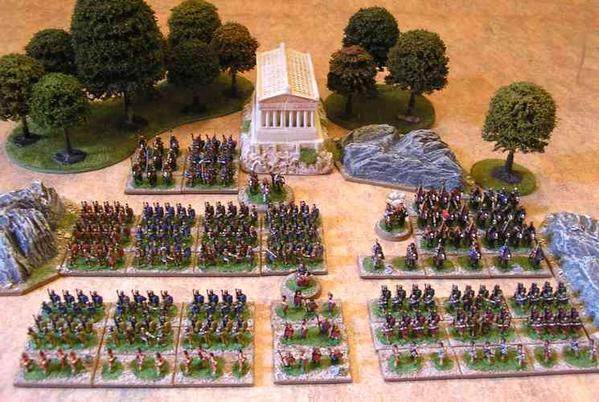
\includegraphics[width=0.8\linewidth]{../ressources/armee_cesar}
	\caption{Exemple d'organisation homogène de l'armée (armée de César - Warmaster ancients \cite{armee_de_cesar})}
	\end{centering}
\end{figure}

Cela permet de construire des formations à grande échelle qui aient une structure prédéfinie.
\begin{figure}[H]
\begin{centering}
\begin{tabular}{| c l | c l | c l | c l |}
	\hline
	\multicolumn{8}{| c |}{\textbf{Armée}}
	\\
	\multicolumn{2}{| c |}{\textbf{Spartiate}} 	& \multicolumn{2}{ c |}{\textbf{Romaine}} & \multicolumn{2}{ c |}{\textbf{Perse}}	& \multicolumn{2}{ c |}{\textbf{Mongole}} 	\\
	\hline
	 					&			& 					&			& 				&			& \textit{Ordu}		& > 10000			\\
	 \itshape Mora 			& 576		& \itshape Légion		& 6000		& \textit{Baivarabam}& 10000		& \textit{Tumen} 	& 10000			\\
	 \itshape Loche			& 144		& \itshape Cohorte		& 600		& \textit{Hazarabam}	& 1000		& \textit{Minghan}  	& 1000			\\
	 \itshape Pentécostye	& 72			& \itshape Manipule		& 200		& \textit{satabam}	& 100		& \textit{Zuut} 		& 100			\\
	 \itshape Énomotie		& 36			& \itshape Centurie		& 100		& \textit{Dathabam} 	& 10			& \textit{Arav} 		& 10				\\
	\hline
\end{tabular}
\caption{Effectif des unités dans différentes armées antiques \cite{mongol_army, spart_army, roman_legion,persian_army}}
\label{tab_army}
\end{centering}
\end{figure}
Comme nous pouvons l'observer sur la figure \ref{tab_army}, les différentes armées sont très hiérarchiques avec souvent quatre niveaux principaux de commandement.


\subsubsection{Contexte}
Les armées interviennent dans deux contextes principaux : la défense de la patrie et la conquête de nouveaux territoires.
\begin{figure}[H]
	\begin{centering}
	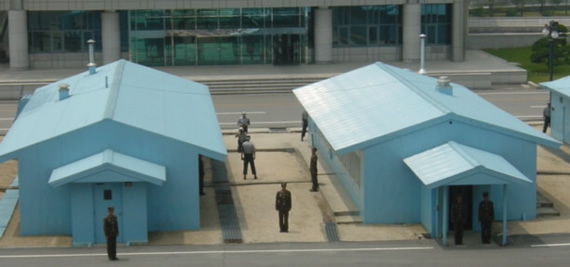
\includegraphics[width=\linewidth]{../ressources/dmz-corea}
	\caption{Zone démilitarisée entre la Corée du Sud et la Corée du Nord \cite{dmz_corea}}
	\end{centering}
\end{figure}
\begin{figure}[H]
	\begin{centering}
	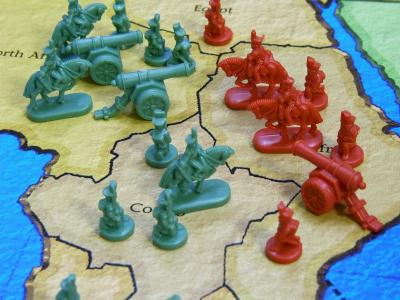
\includegraphics[scale=0.8]{../ressources/risk-board-game}
	\caption{Tentative de conquête dans le jeu Risk \cite{risk_picture}}
	\end{centering}
\end{figure}




\subsection{Guérillas}
Les guérillas se forment à la suite d'une scission idéologique entre le pouvoir en place et une partie de la population. Elles ont souvent à leur tête un leader charismatique.

\subsubsection{Structure}
Ces organisation sont souvent structurées de façon très hétérogène : peu de responsables et des formations à petite échelle.
\begin{figure}[H]
	\begin{centering}
	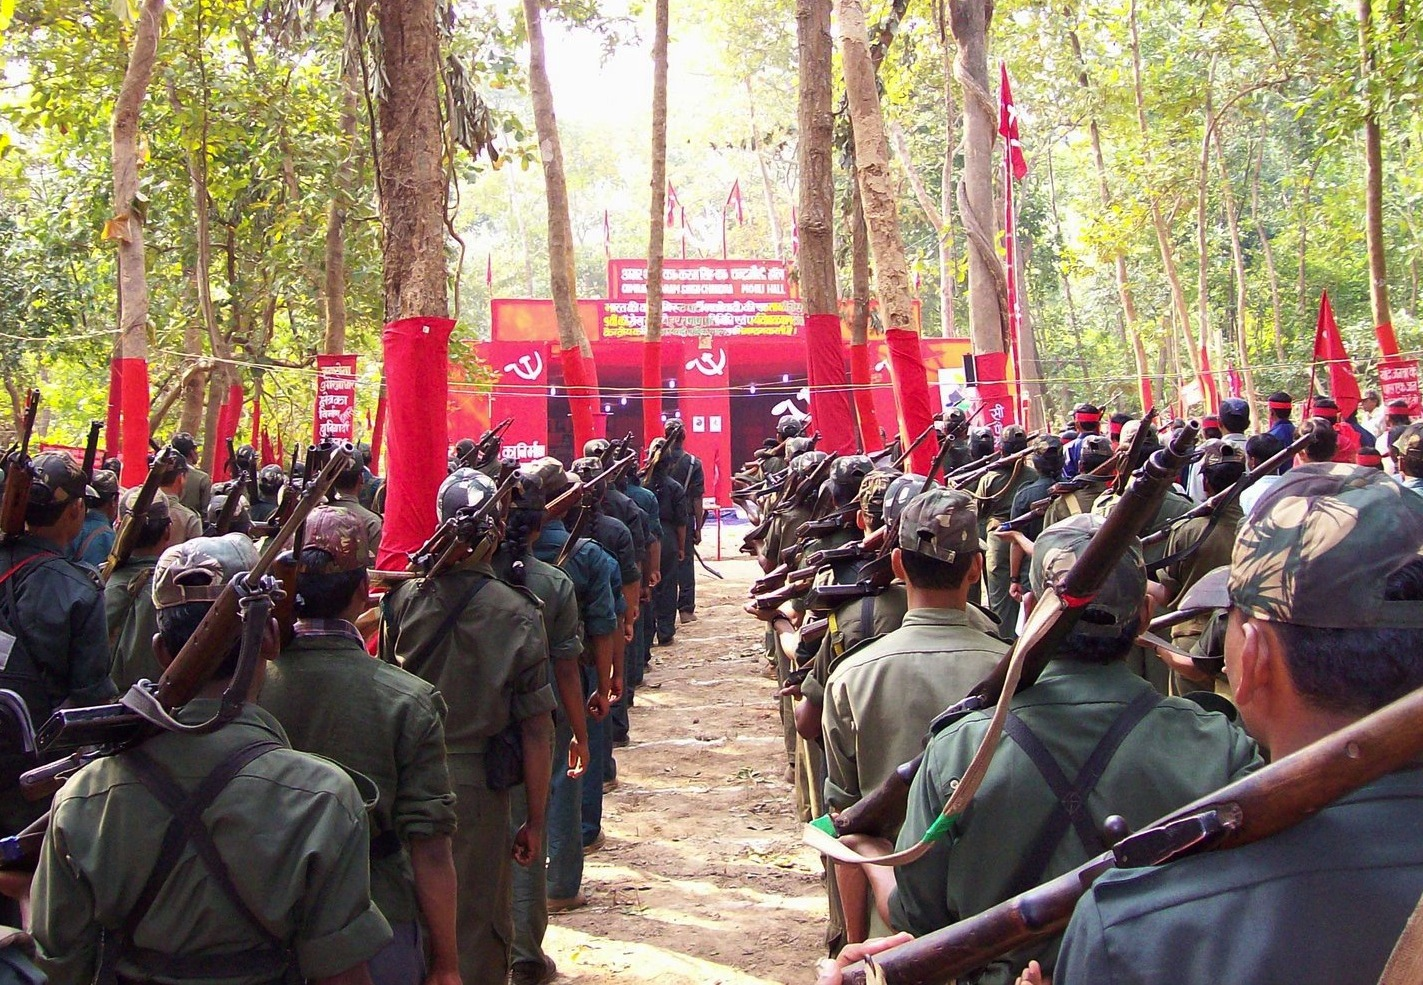
\includegraphics[width=\linewidth]{../ressources/guerrilla_naxalite}
	\caption{Guérilla Naxalite (Inde) \cite{guerrilla_naxalite}}
	\end{centering}
\end{figure}

Les guérillas, comme le montre la figure \ref{tab_guerrilla}, ont une échelle réduite par rapport aux forces contre lesquelles elles luttent.
\begin{figure}[H]
	\begin{centering}
	\begin{tabular}{| l | c | c | c | c |}
	\hline
	\textbf{Localisation}		& \textbf{Irlande} 	& \textbf{Inde} 	& \textbf{Cuba}	& \textbf{Colombie}	\\
	\hline
	\textbf{Régime}			& 55.000			& 1.414.000	& 35.000		& 300.000			\\
	\textbf{Insurgés}		& 15.000			& 15.000		& 200		& 20.000			\\
	\hline
	\end{tabular}
	\caption{Effectifs des forces du régime par rapport aux forces des guérillas \cite{naxalite_guerrilla_wiki, irish_civil_war_wiki}}
	\label{tab_guerrilla}
	\end{centering}
\end{figure}


\subsubsection{Contexte}
Les guérilla se forment dans des contextes de guerre civile afin de renverser le pouvoir en place. Les forces de guérilla sont adaptées au terrain : montagnes, maquis, villes \ldots
\begin{figure}[H]
	\begin{centering}
	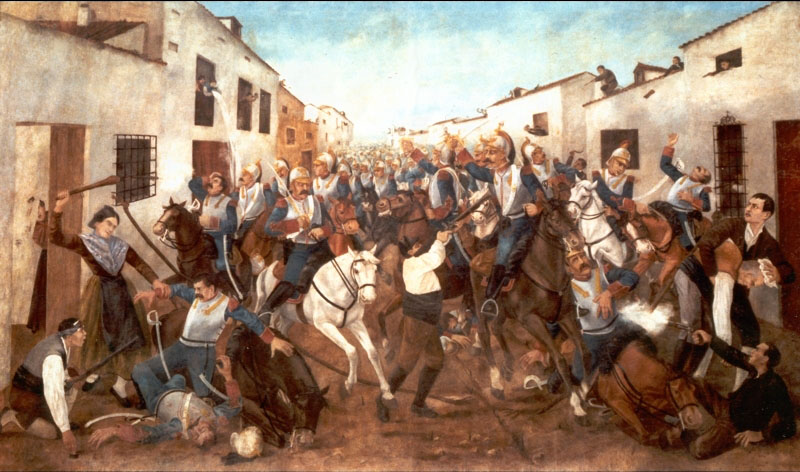
\includegraphics[width=\linewidth]{../ressources/valdepenas}
	\caption{Soulèvement de Valdepeñas ; guérilla urbaine \cite{valdepenas}}
	\end{centering}
\end{figure}
Elles sont mobiles.
\begin{figure}[H]
	\begin{centering}
	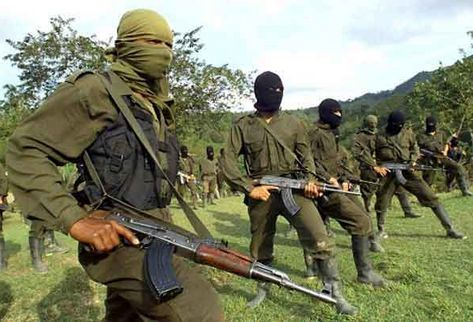
\includegraphics[]{../ressources/guerrilla_colombia}
	\caption{Guérilla colombienne \cite{guerrilla_colombia}}
	\end{centering}
\end{figure}
La plupart des recrues sont des civils.
\begin{figure}[H]
	\begin{centering}
	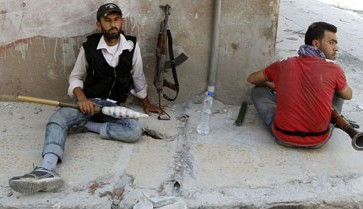
\includegraphics[]{../ressources/rebel_syrie}
	\caption{Des rebelles en Syrie \cite{rebel_syrie}}
	\end{centering}
\end{figure}


\section{Stratégies militaires}

\subsection{Définitions}
Politique \cite{politique_jomini}
\begin{quote}“La politique de la guerre c’est tout simplement décider où, quand, comment, avec quels alliés et pourquoi entrer en guerre.”\end{quote}
\begin{figure}[H]
	\begin{centering}
	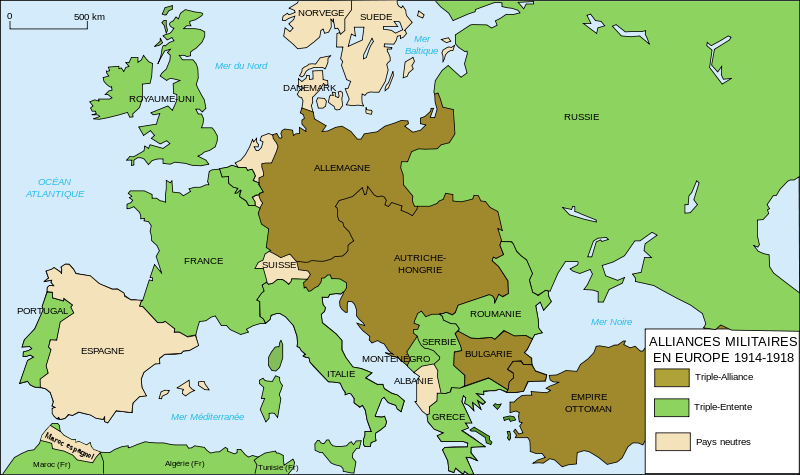
\includegraphics[width=0.95\linewidth]{../ressources/alliances_ww1}
	\caption{Alliances militaires en Europe 1914-1918 \cite{ww1}}
	\end{centering}
\end{figure}

Stratégie \cite{military_strategy}
\begin{quote}“La stratégie militaire est l'art de coordonner -au plus haut niveau de décision- l'action de l'ensemble des forces militaires de la Nation pour conduire une guerre, gérer une crise ou préserver la paix.”\end{quote}
\begin{figure}[H]
	\begin{centering}
	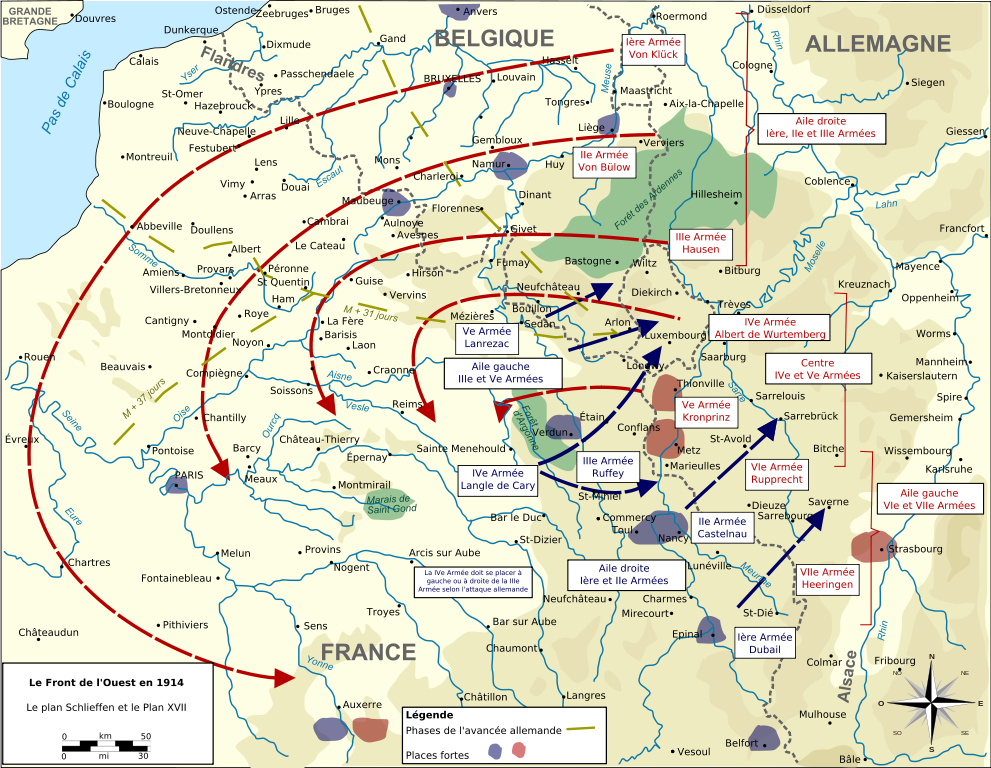
\includegraphics[width=\linewidth]{../ressources/strategy_ww1}
	\caption{Plans de bataille des états-majors allemand et français pendant la WW1 \cite{ww1}}
	\end{centering}
\end{figure}

Tactique \cite{tactic}
\begin{quote}“La tactique est l'art de diriger une bataille, en combinant, par la manœuvre, l'action des différents moyens de combat en vue d'obtenir le maximum d'efficacité.”\end{quote}
\begin{figure}[H]
	\begin{centering}
	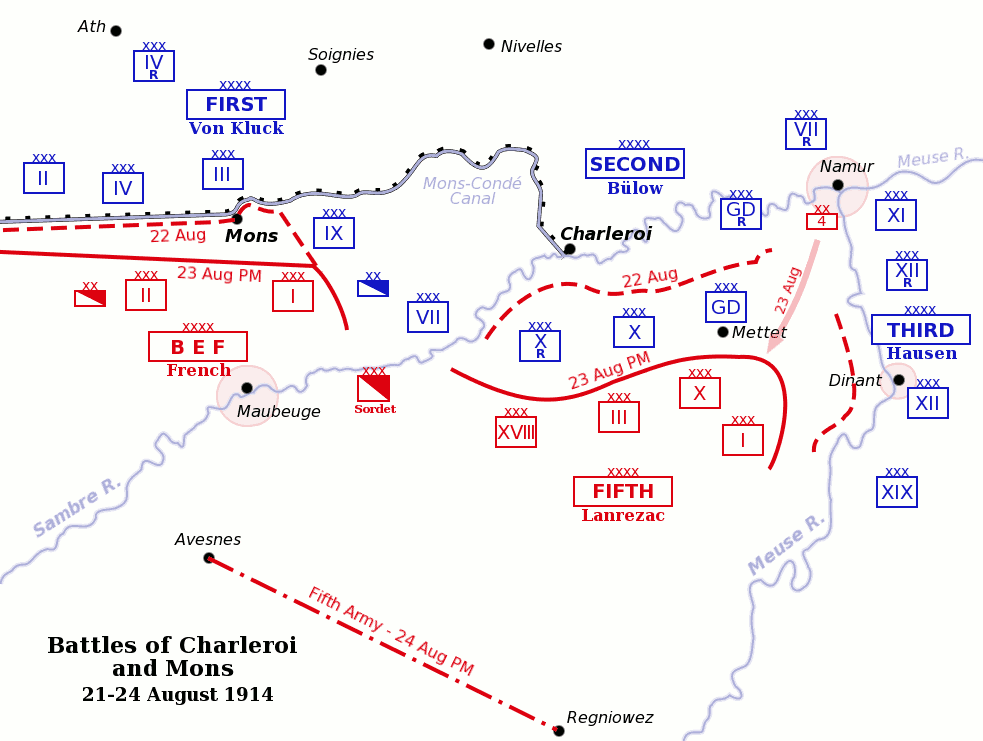
\includegraphics[width=\linewidth]{../ressources/Battles_of_Charleroi_ww1}
	\caption{Mouvement de troupes pendant la bataille de Charleroi (WW1) \cite{charleroi_battle}}
	\end{centering}
\end{figure}



\subsection{Stratégies}

\subsubsection{Sun Tzu}
Sun Tzu était un général chinois du \siecle{6} BC \cite{sun_tzu_wiki} dont la stratégie se résumait pas la citation suivante : \begin{quote}“L'art de la guerre, c'est de soumettre l'ennemi sans combat.”\end{quote}
\begin{figure}[H]
	\begin{centering}
	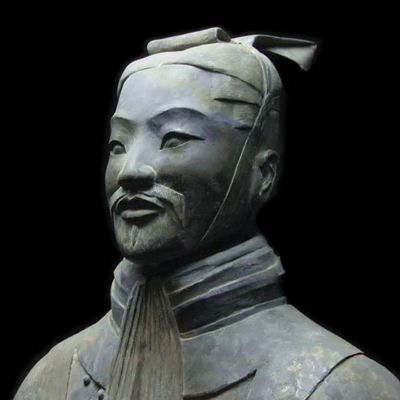
\includegraphics[width=5cm]{../ressources/sun_tzu_general}
	\caption{Sun Tzu \cite{sun_tzu_fighting}}
	\end{centering}
\end{figure}

Son ouvrage \emph{L'art de la guerre} \cite{tzu1997art} a traversé les siècles et nous inculque les préceptes suivants. L'art de la guerre se résume en deux concepts de base : prendre toutes les possessions de l'adversaire et les conserver intactes afin de s'en trouver renforcé ; engager des forces anodines pour faciliter la victoire par l'adaptabilité, la préparation, la connaissance du terrain et des forces en présence (espionnage).

Les cinq éléments suivants sont à prendre en compte pour élaborer une stratégie :
\begin{enumerate}
\item cause morale
\item conditions climatiques
\item conditions géographiques
\item qualités du dirigeant
\item organisation et discipline
\end{enumerate}



\subsubsection{Alexandre le grand}
Alexandre le grand était un roi de Macédoine (Grèce) vivant au \siecle{4} BC. Nous avons souhaité illustrer sa stratégie par cette citation : \begin{quote}“Ce qui ne me tue pas me rend plus fort.”\end{quote}
\begin{figure}[H]
	\begin{centering}
	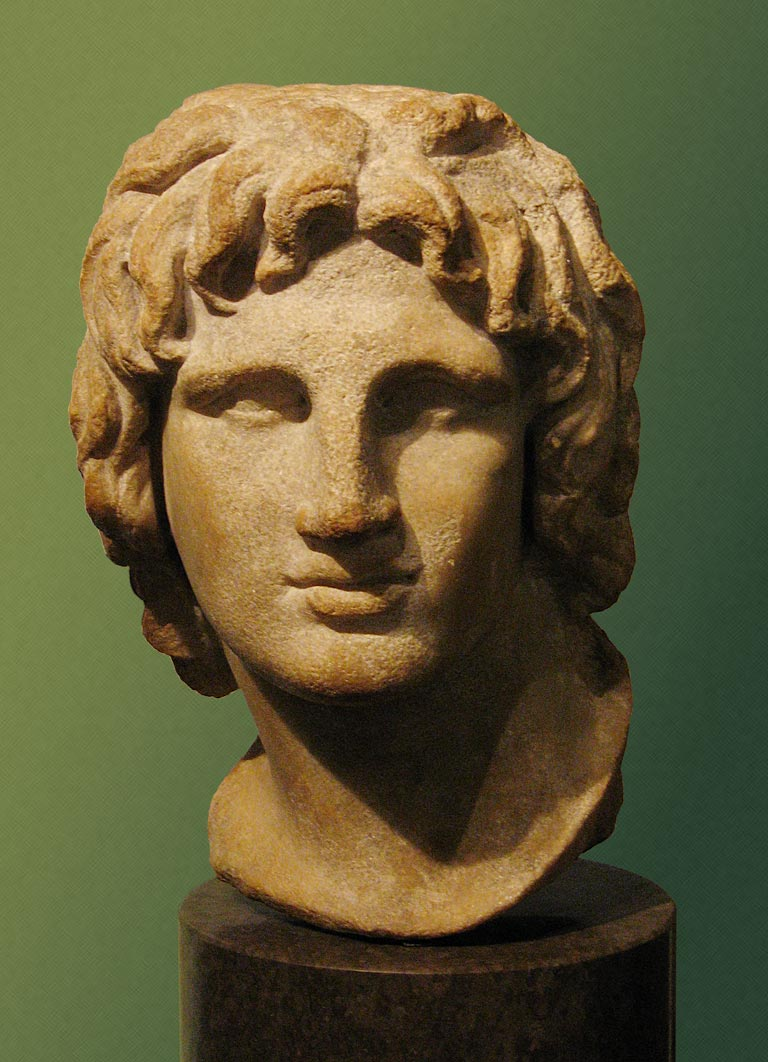
\includegraphics[width=5cm]{../ressources/AlexanderTheGreat_Bust}
	\caption{Alexandre le grand \cite{alexander_the_great}}
	\end{centering}
\end{figure}

Les principes fondateurs de sa stratégie sont la conscription et l'intégration des peuples vaincus et l'allègement de l'équipement des troupes.

Lors de l'élaboration d'une stratégie, nous pouvons retenir d'Alexandre le grand les axes suivants \cite{alexandre_balkans} :
\begin{enumerate}
\item assurer ses arrières
\item choisir judicieusement la voie d'accès pour chaque conquête
\end{enumerate}


\subsubsection{Julius Caesar}
Julius Caesar était un général, homme politique et écrivain romain (Italie) vivant au \siecle{1} BC. Sa stratégie est illustrée par la citation suivante : \begin{quote}“L’expérience, voilà le maître en toutes choses.”\end{quote}
\begin{figure}[H]
	\begin{centering}
	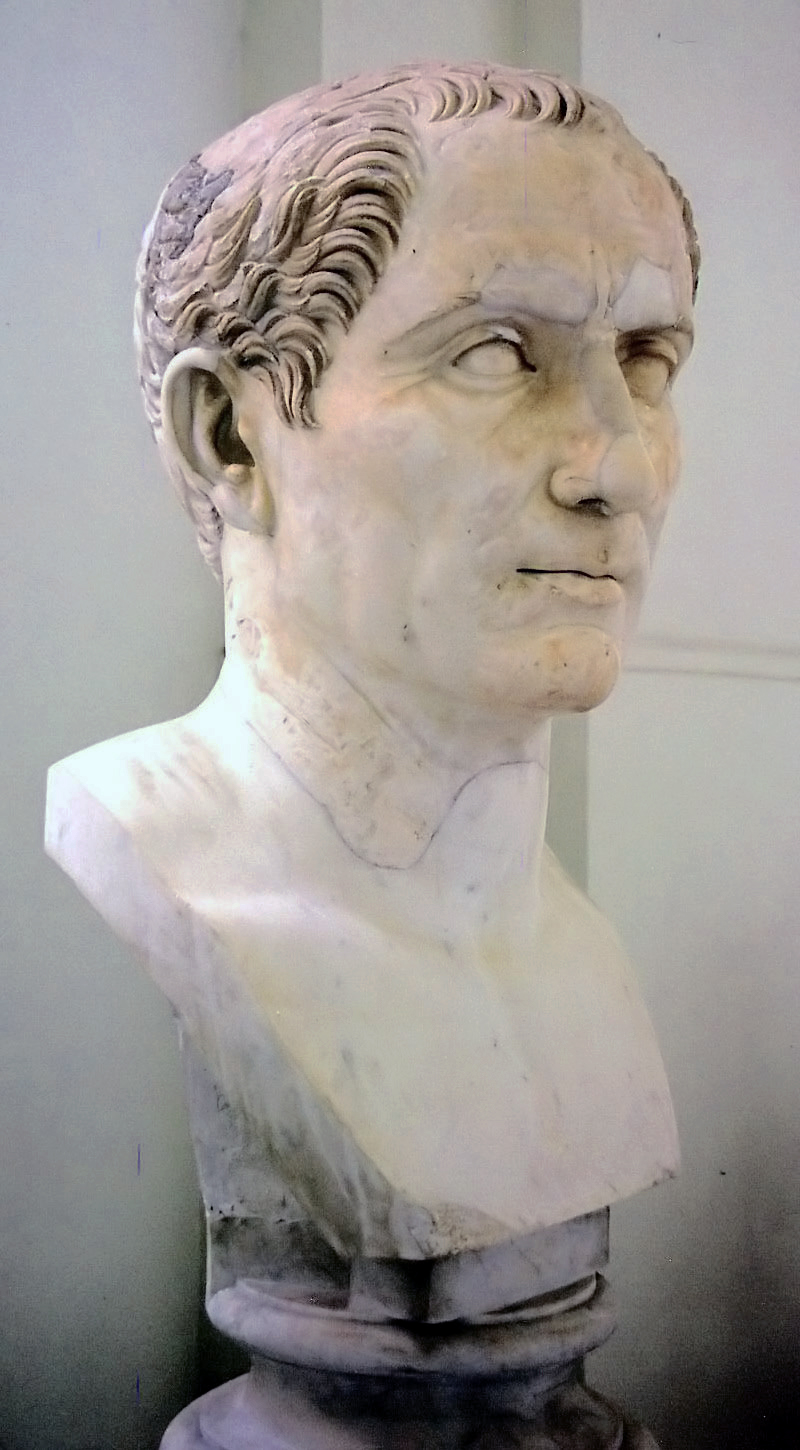
\includegraphics[width=5cm]{../ressources/cesare}
	\caption{Julius Caesar \cite{caesar_wiki}}
	\end{centering}
\end{figure}

Sa stratégie reposait avant tout sur la stabilité militaire et logistique. Il nous a enseigné l'importance des axes stratégiques suivants \cite{caesar_lacks} :
\begin{enumerate}
\item l'utilisation de l'infanterie lourde
\item les bataillons étrangers spécialisés
\item le choix judicieux des formations en fonction des conditions géographiques
\item la construction de bivouacs fortifiés
\end{enumerate}


\subsubsection{Genghis Khan}
De son premier nom Temüdjin, fondateur de l'empire Mongol au \siecle{12}.
\begin{figure}[H]
	\begin{centering}
	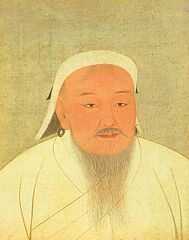
\includegraphics[width=5cm]{../ressources/genghis_khan}
	\caption{Genghis Khan \cite{khan_wiki}}
	\end{centering}
\end{figure}
La meilleure arme de l'armée mongole était la terreur et Genghis Khan l'illustre de la manière suivante : \begin{quote}“Le plus grand bonheur du Mongol est de vaincre l’ennemi, de ravir ses trésors, de faire hurler ses serviteurs, de se sauver au galop de ses chevaux bien nourris [\ldots]”\end{quote}
Les mongoles étaient un peuple nomade organisé en tribus qui fut réuni par Genghis Khan. Ses principales armes furent la guerre psychologique, le règne de la terreur et la connaissance du terrain à travers l'espionnage et un grande quantité d'éclaireurs \cite{military_strategy}.

Nous pouvons résumer les grandes lignes de sa stratégie de la manière suivante \cite{mongol_army} :
\begin{enumerate}
\item peu de troupes et une avant-garde forte
\item des troupes montées rapides qui pouvaient manger leurs chevaux en cas de besoin
\item la délégation des décisions à ses seconds
\item de nombreux (et bien placés) relais de communication et de ravitaillement
\item attaques biologiques (catapultes lançant les corps en décomposition des ennemis)
\end{enumerate}


\subsubsection{Napoléon Bonaparte}
Napoléon Bonaparte était le premier empereur des Français au \siecle{18}. Il fut le général français le plus expansionniste. Sa stratégie était basée sur le fait de percer la défense adverse le plus rapidement possible, ainsi disait-il : \begin{quote}“Réunir ses feux contre un seul point ; une fois la brèche faite, l’équilibre est rompu, tout le reste devient inutile.”\end{quote}
\begin{figure}[H]
	\begin{centering}
	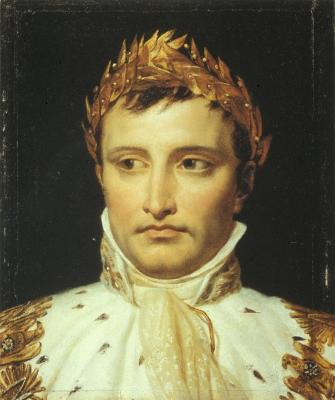
\includegraphics[width=5cm]{../ressources/napoleon}
	\caption{Napoléon Bonaparte \cite{napoleon_portrait}}
	\end{centering}
\end{figure}

Les principes fondateurs selon lui sont : la recherche systématique de la bataille et la destruction totale des forces adverses ; ainsi on peut être le plus fort à l’endroit où l’on a décidé de frapper le coup décisif \cite{napoleon_wiki}.

Les principaux axes stratégiques \cite{napoleon} que l'on peut retenir sont :
\begin{enumerate}
\item vitesse de manœuvre : \emph{Blitzkrieg}
\item fortifications
\item lignes de réapprovisionnement provisoires
\item artillerie
\end{enumerate}


\subsubsection{Conclusion}
Si l'on essaie d'analyser les stratégies examinées précédemment, nous pouvons les regrouper en deux types : stratégies directes et stratégies indirectes.

\begin{tabular}{|p{0.45\linewidth}|p{0.45\linewidth}|}
\hline
\emph{Stratégie indirecte} & \emph{Stratégie directe}\\
\hline
renseignement & conscription\\
embuscade & recherche de la bataille décisive\\
tromperie & planification et formations\\
sabotage & fortifications\\
\hline
\end{tabular}

\begin{figure}[H]
	\begin{centering}
	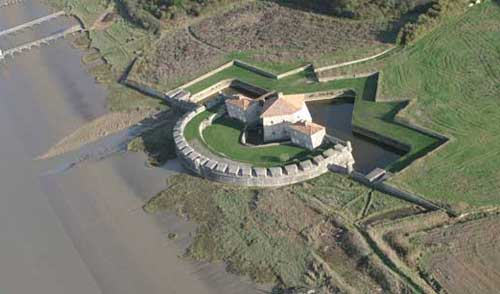
\includegraphics[width=0.8\linewidth]{../ressources/Vauban_Fort_Lupin}
	\caption{Vue aérienne du Fort Lupin construit par Vauban (Rochefort). \cite{fort_lupin}}
	\end{centering}
\end{figure}
\begin{figure}[H]
	\begin{centering}
	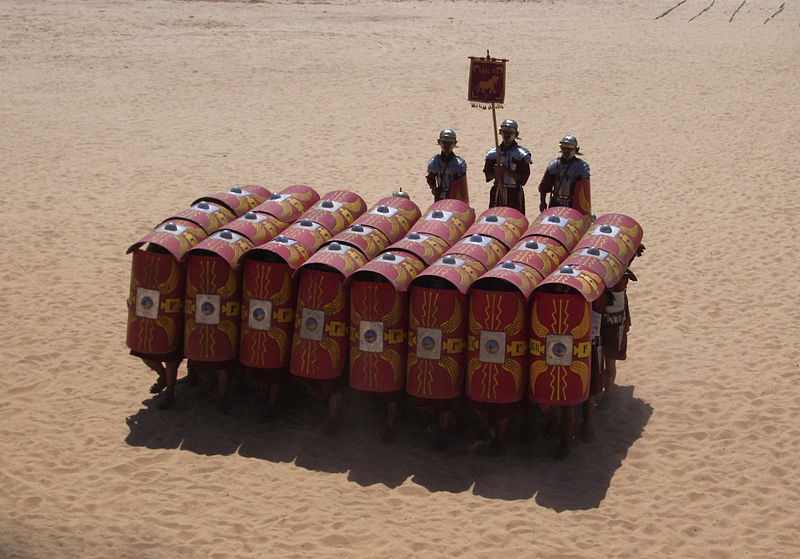
\includegraphics[width=\linewidth]{../ressources/tortue}
	\caption{La tortue : formation défensive romaine. \cite{turtle_form}}
	\end{centering}
\end{figure}
\begin{figure}[H]
	\begin{centering}
	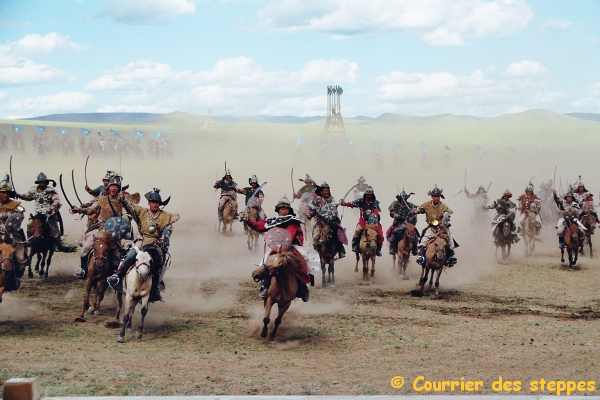
\includegraphics[width=\linewidth]{../ressources/mongol_army}
	\caption{Charge de cavalerie mongole. \cite{mongol_cavalery}}
	\end{centering}
\end{figure}
\begin{figure}[H]
	\begin{centering}
	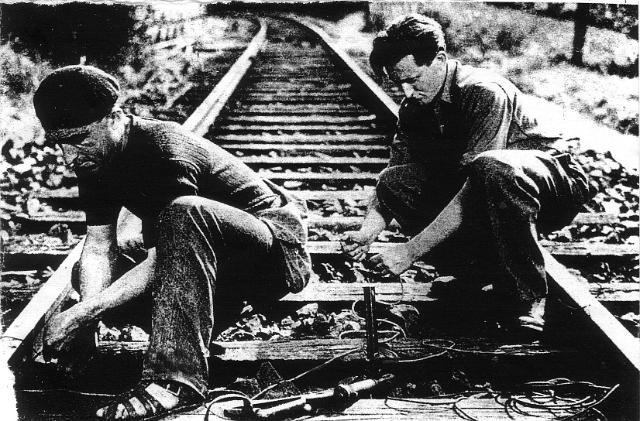
\includegraphics[width=\linewidth]{../ressources/sabotage_maquisards}
	\caption{Sabotage d'une voie de chemin de fer - guerre de 1914. \cite{sabotage}}
	\end{centering}
\end{figure}
\cite{war}


\subsection{Formations et unités}

\subsubsection{Infanterie}
\begin{figure}[H]
	\begin{centering}
	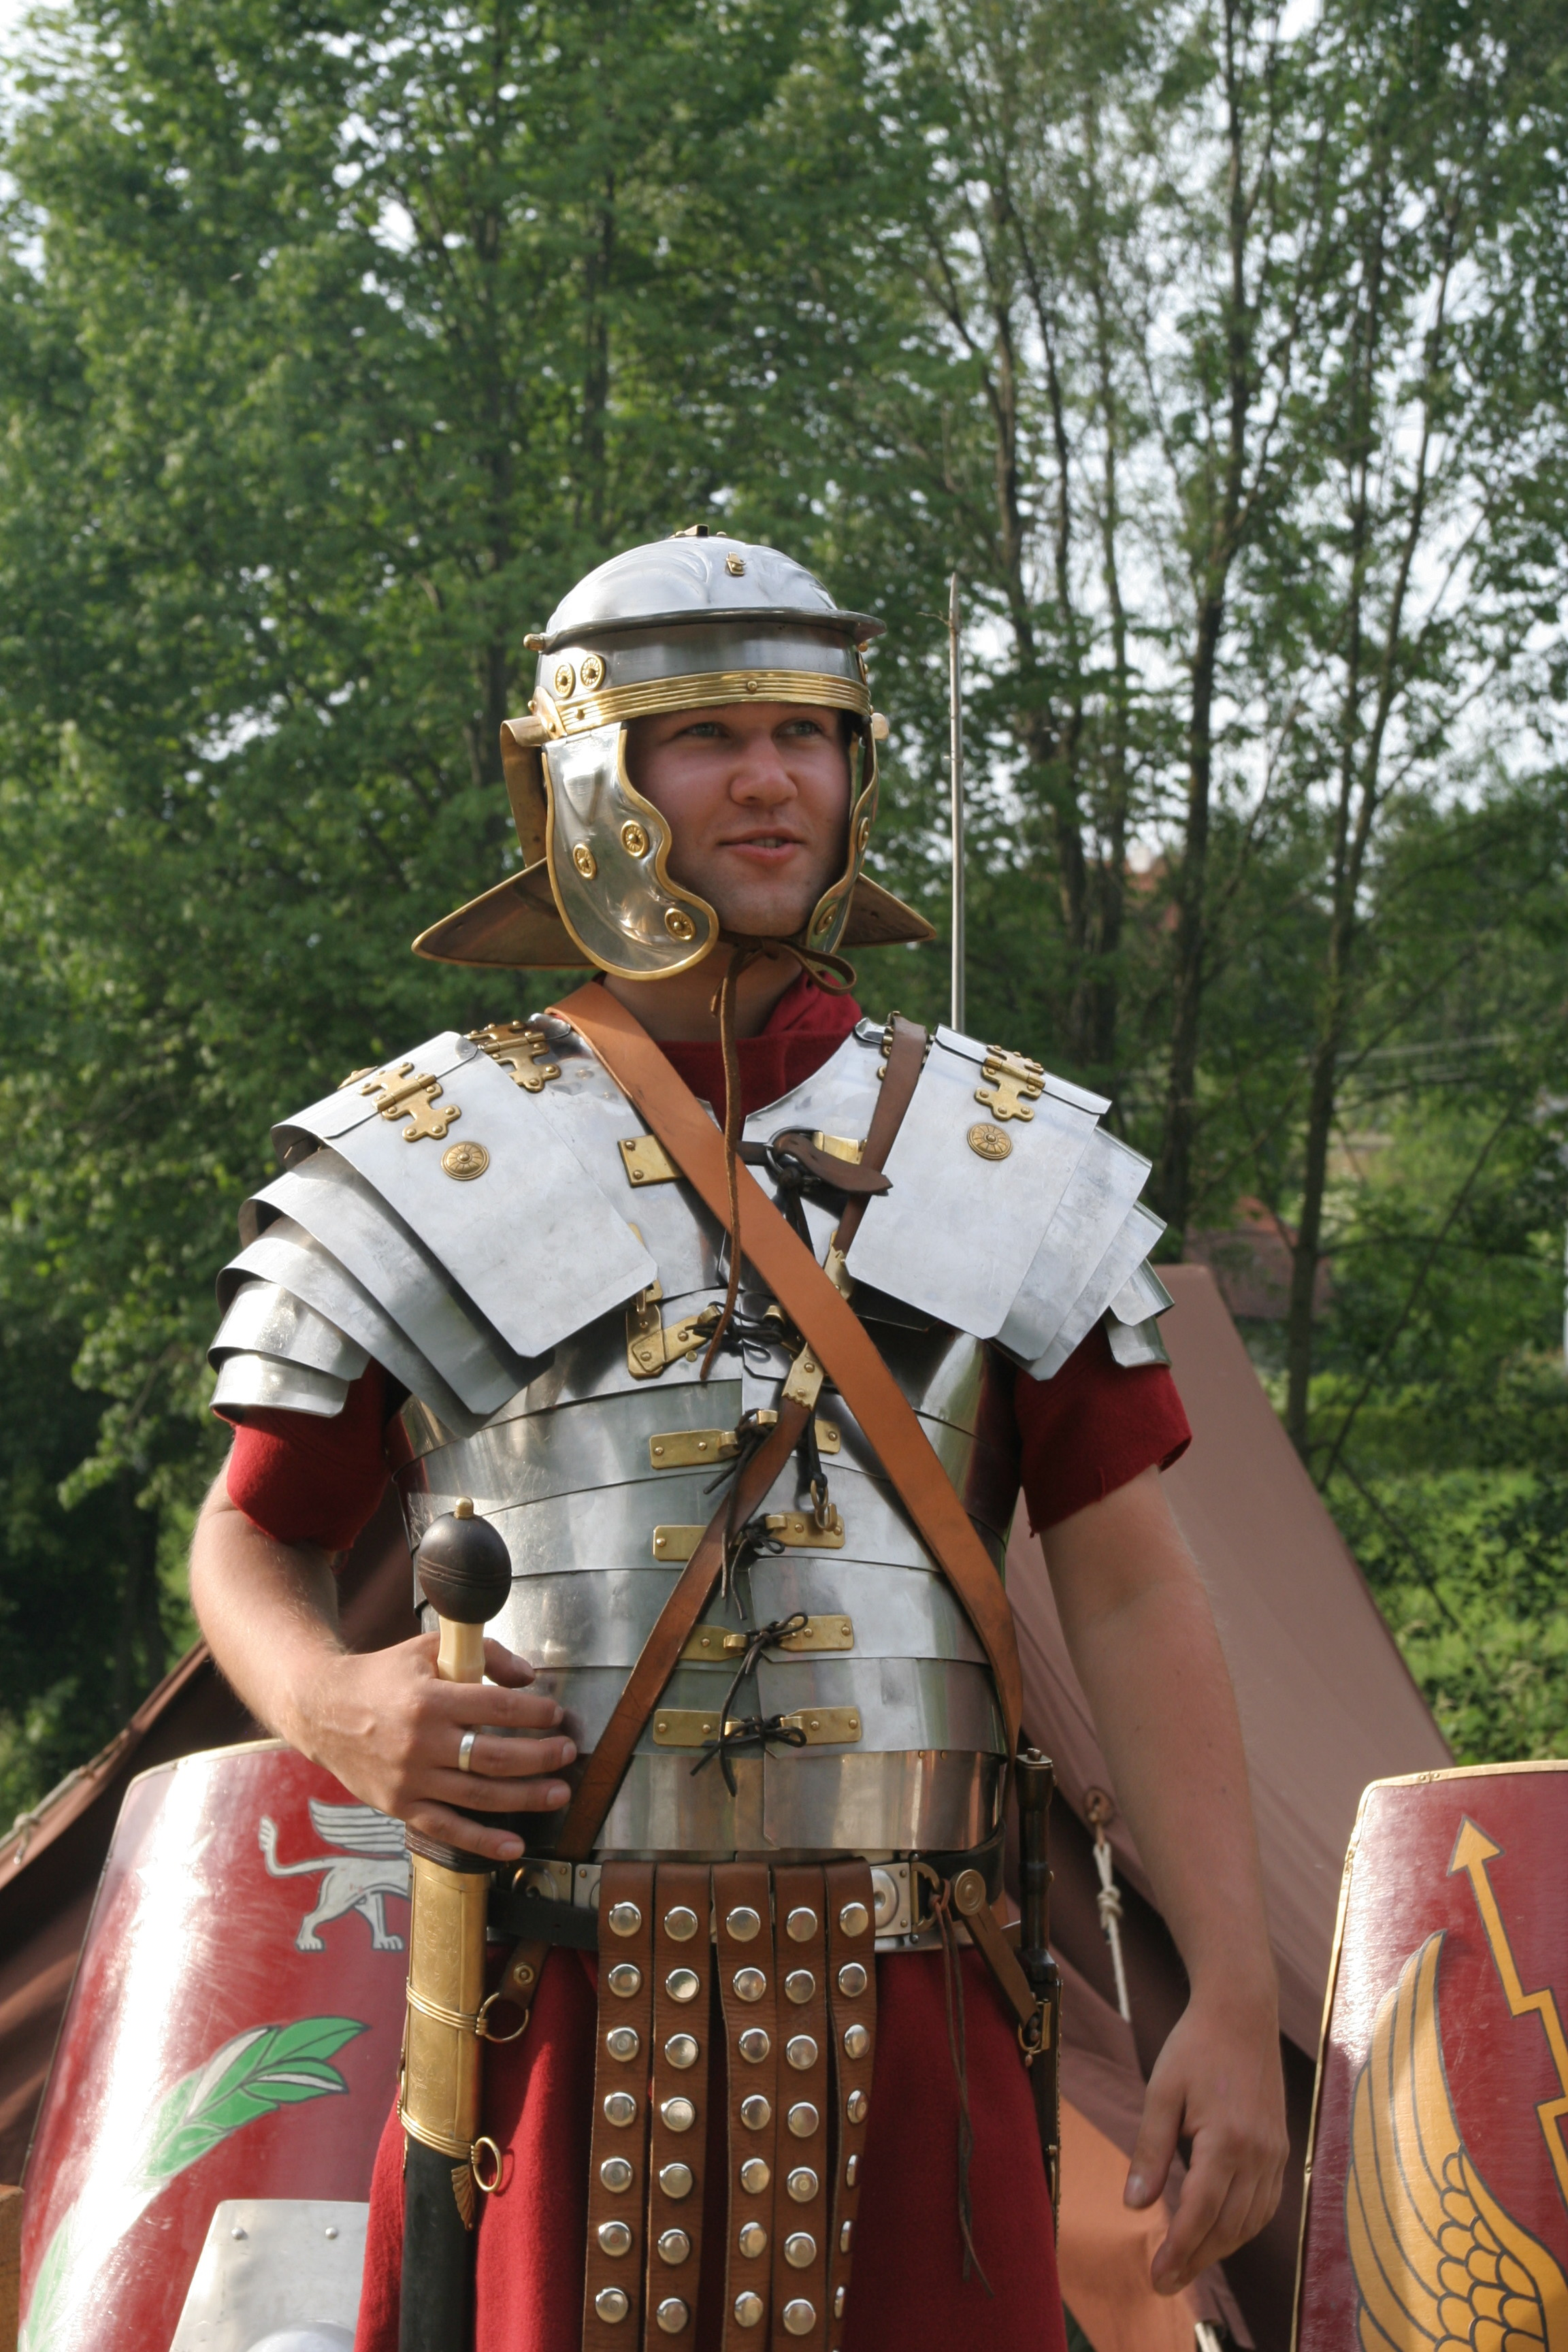
\includegraphics[width=0.42\paperwidth]{../ressources/Roman_soldier}
	\caption{Uniforme d'un légionnaire romain du \siecle{1} siècle. \cite{infantery}}
	\end{centering}
\end{figure}
\begin{figure}[H]
	\begin{centering}
	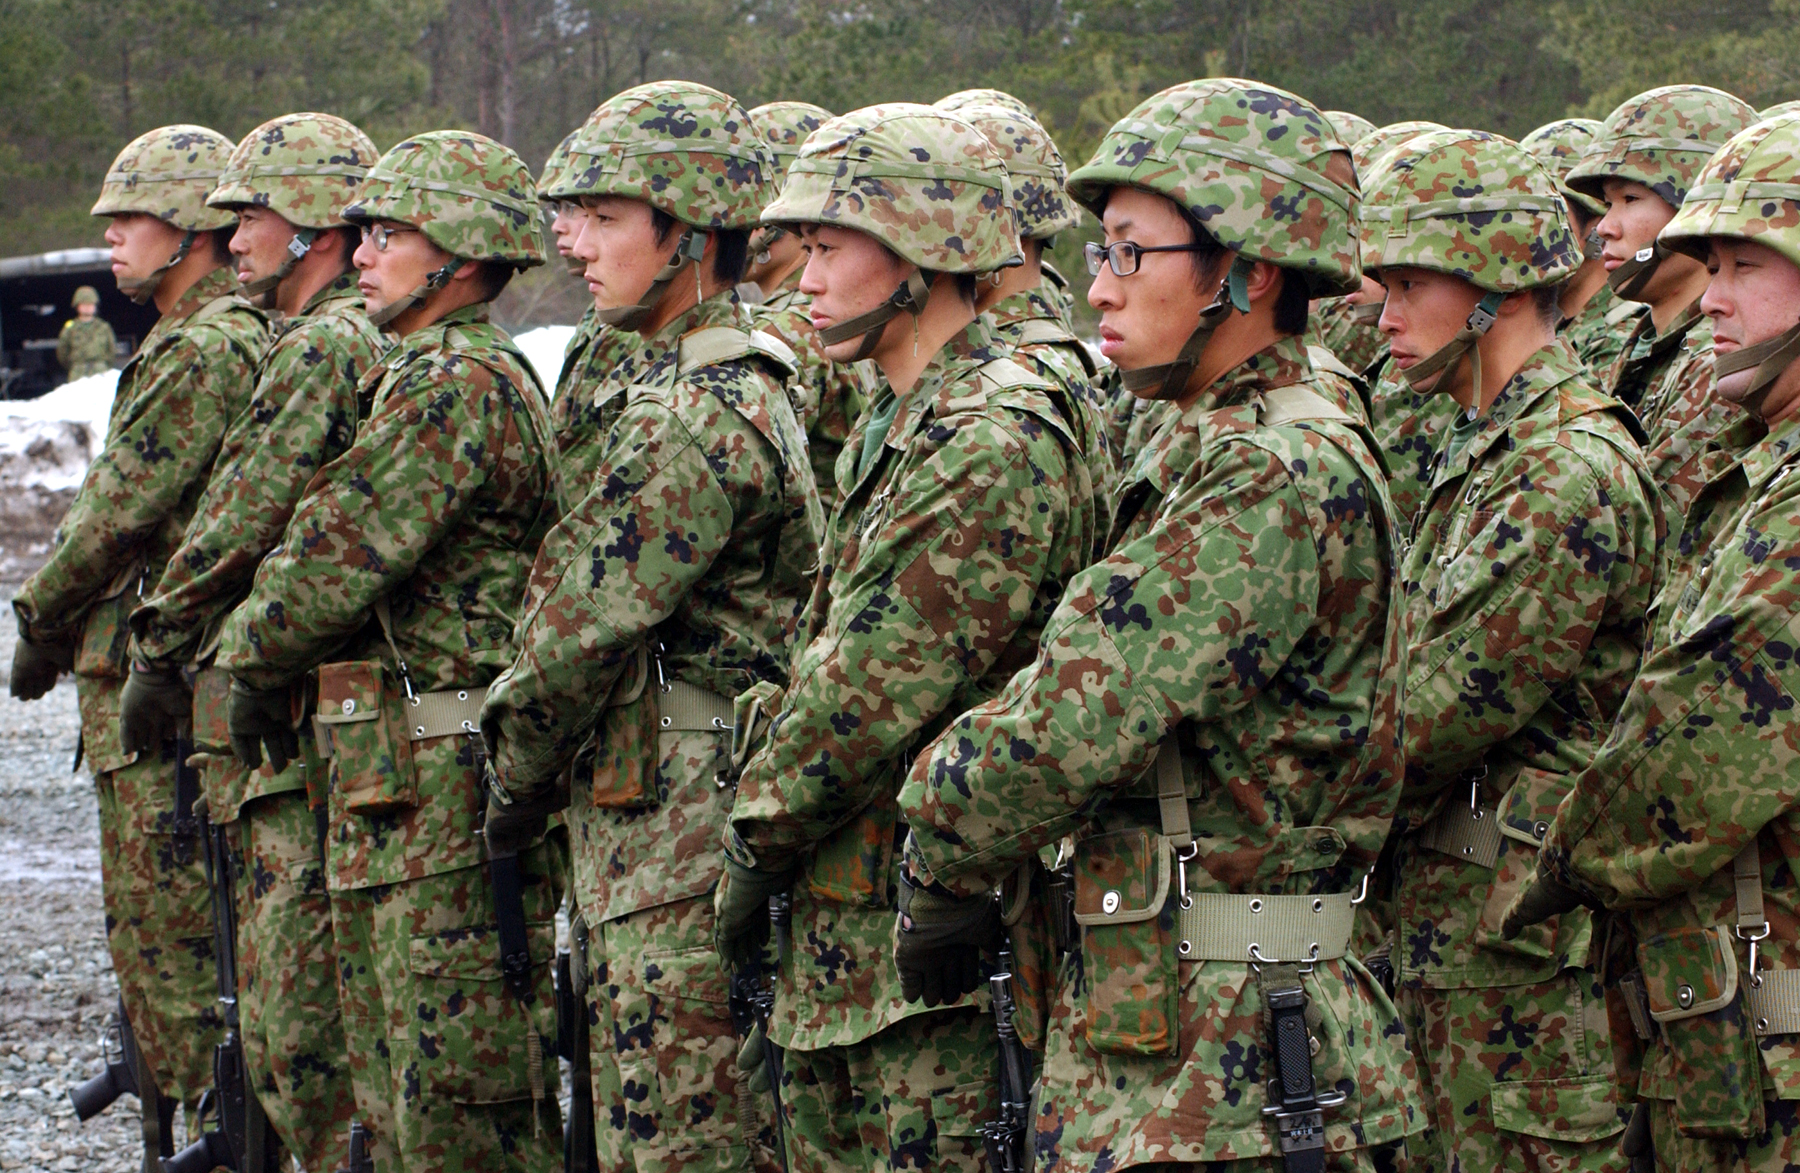
\includegraphics[width=0.55\paperwidth]{../ressources/JGDSF_Soldiers}
	\caption{Japan Ground Self-Defense Force infantry. \cite{infantery}}
	\end{centering}
\end{figure}

\subsubsection{Cavalerie légère}
\begin{figure}[H]
	\begin{centering}
	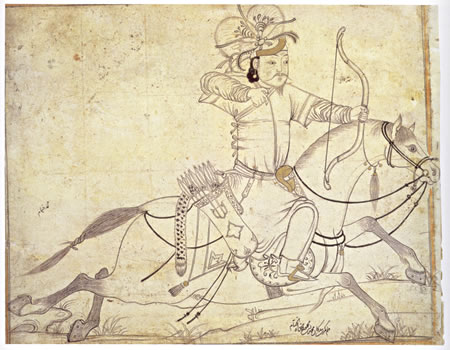
\includegraphics[width=0.5\paperwidth]{../ressources/IlkhanidHorseArcher}
	\caption{Archer à cheval Houlagides. \cite{archery}}
	\end{centering}
\end{figure}
\begin{figure}[H]
	\begin{centering}
	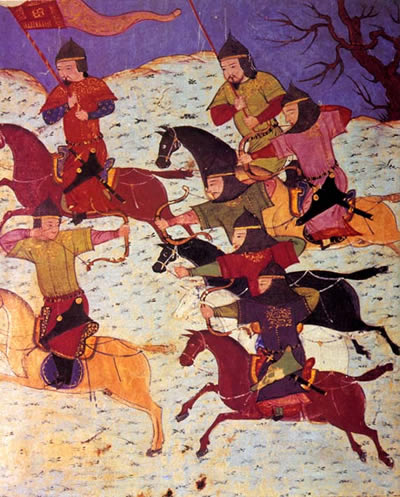
\includegraphics[width=0.47\paperwidth]{../ressources/MongolCavalrymen}
	\caption{Archers mongoles à cheval au combat (illustration d'un manuscrit du début du xive siècle) \cite{mongol_army}}
	\end{centering}
\end{figure}


\subsubsection{Cavalerie lourde}
\begin{figure}[H]
	\begin{centering}
	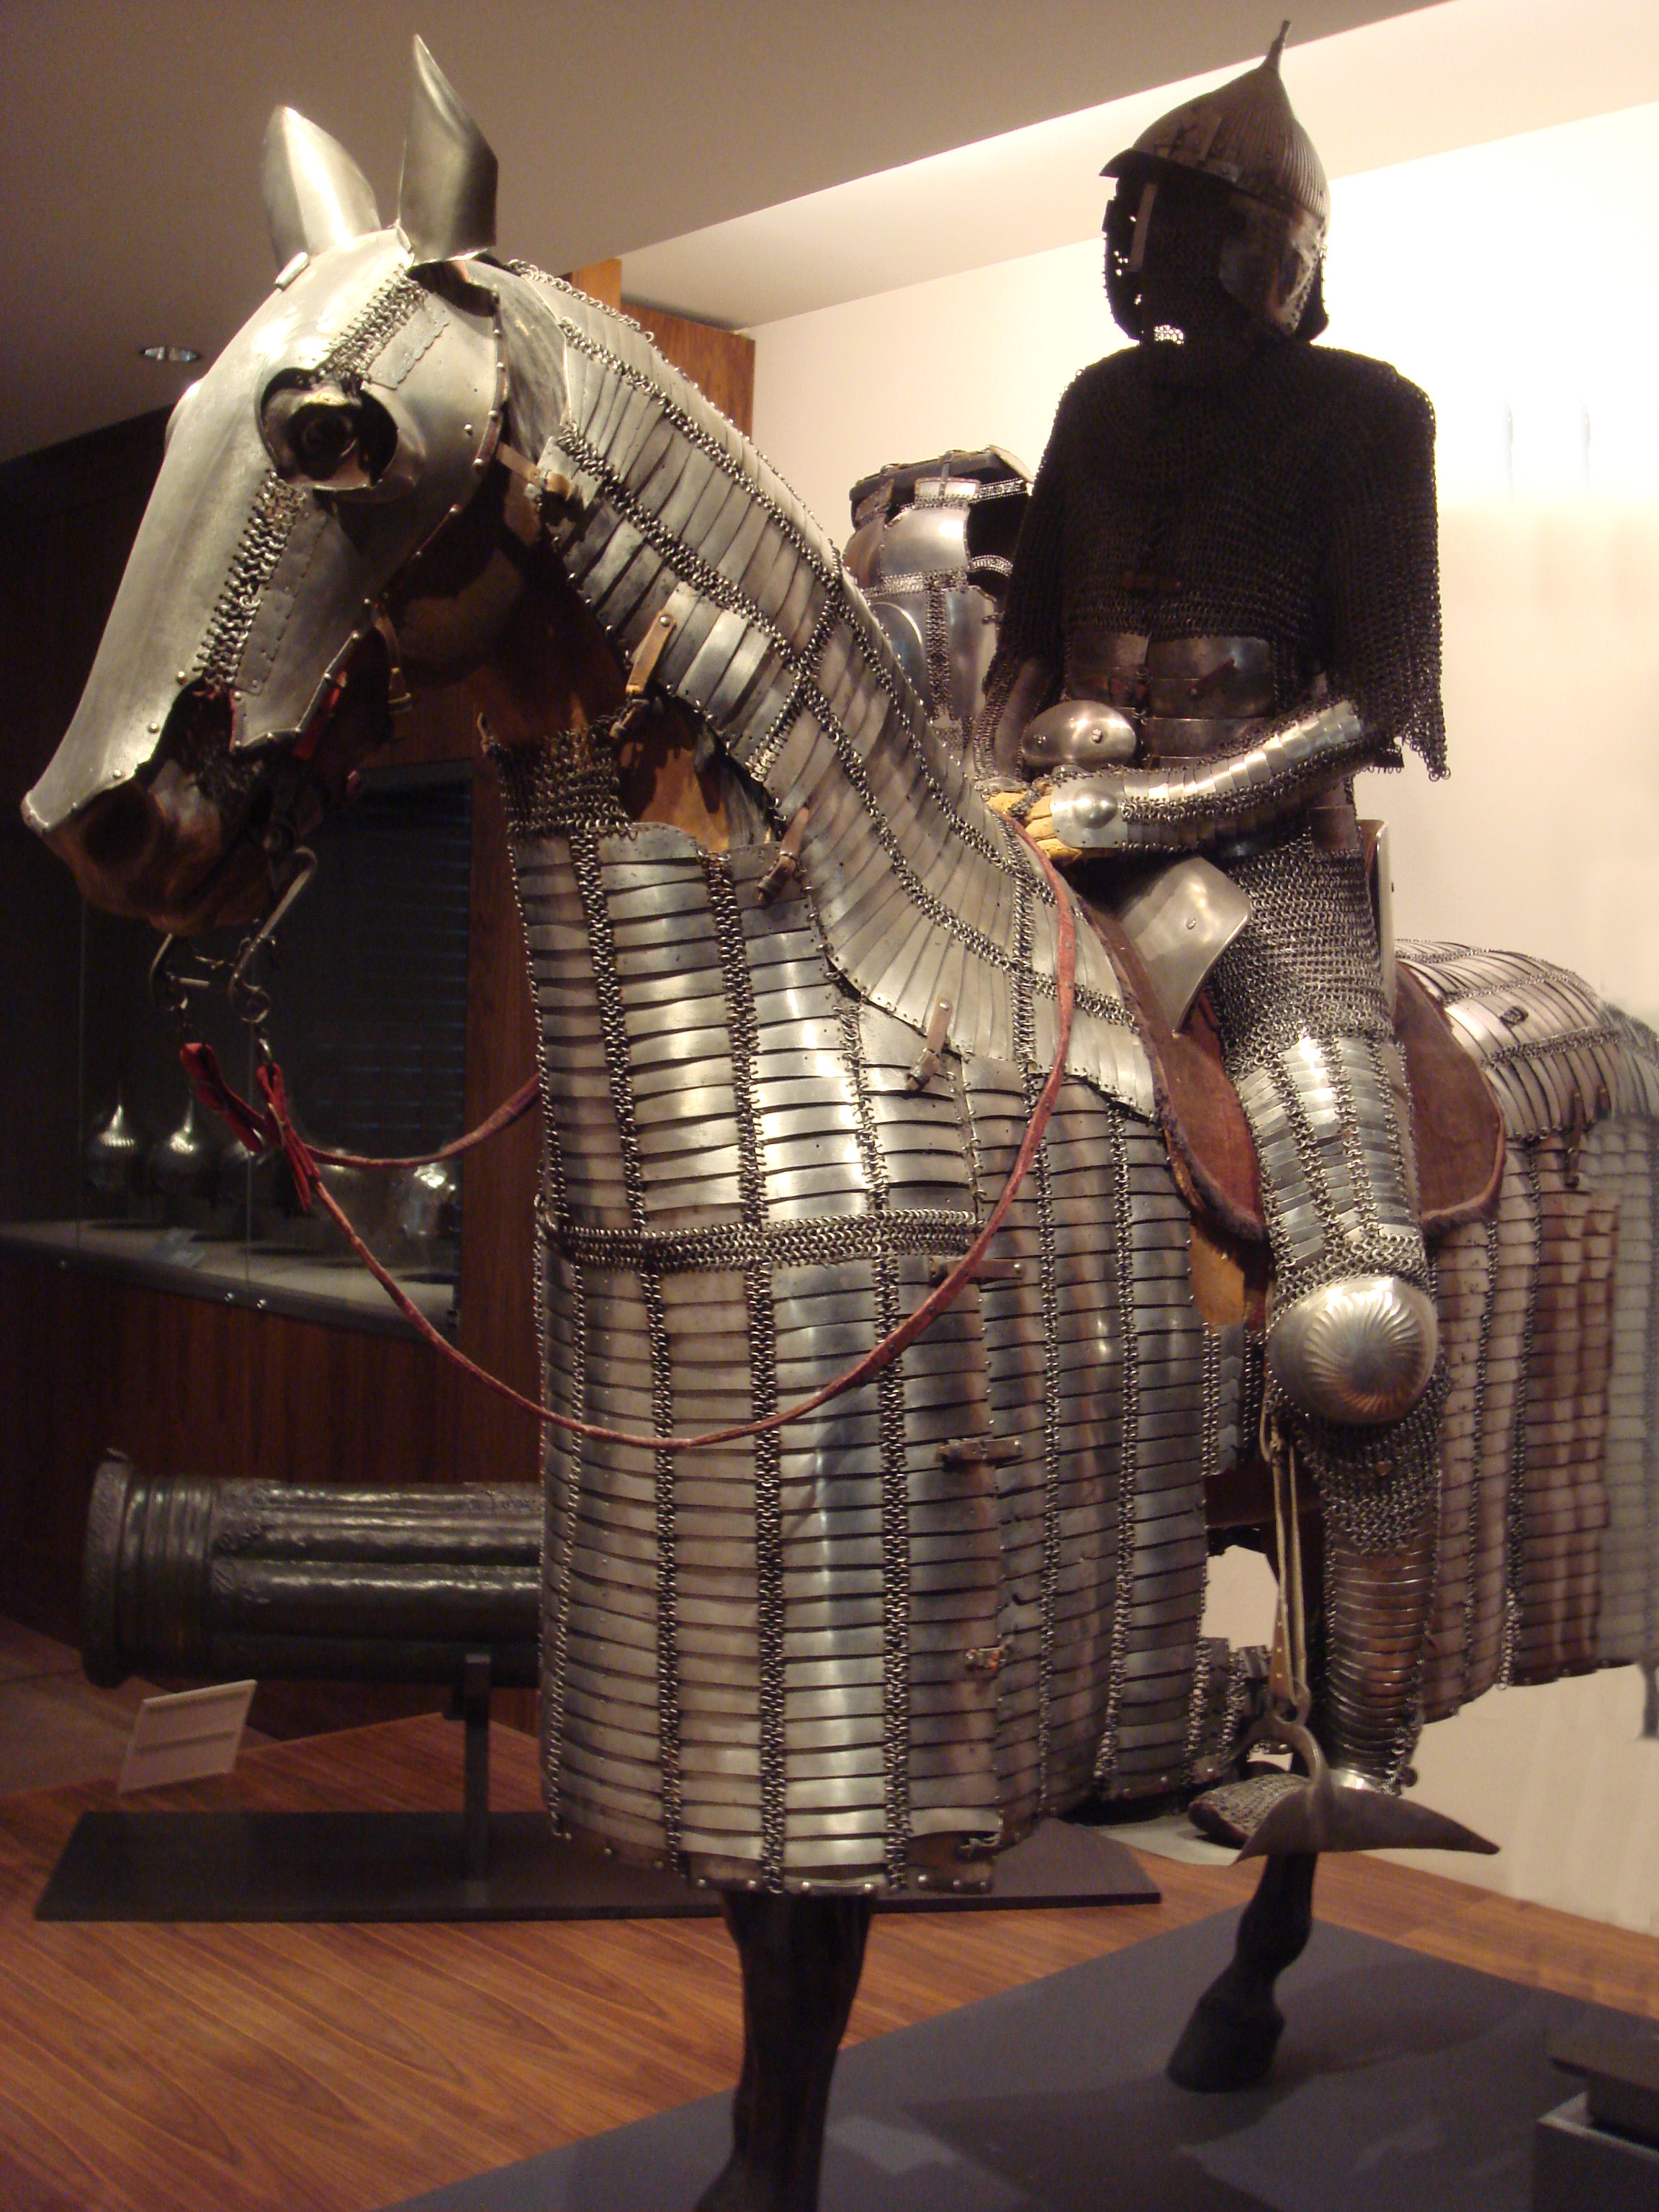
\includegraphics[width=0.44\paperwidth]{../ressources/Ottoman_Mamluk_horseman}
	\caption{Ottoman Mamluk heavy cavalry, circa 1550. \cite{heavy_cavalry}}
	\end{centering}
\end{figure}
\begin{figure}[H]
	\begin{centering}
	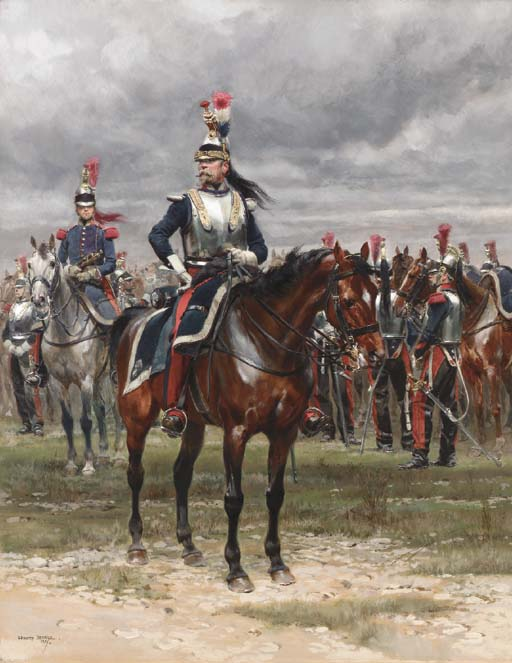
\includegraphics[width=0.5\paperwidth]{../ressources/cuirassiers}
	\caption{French cuirassiers, 19th century \cite{heavy_cavalry}}
	\end{centering}
\end{figure}

\subsubsection{Formation en triple ligne}
\begin{figure}[H]
	\begin{centering}
	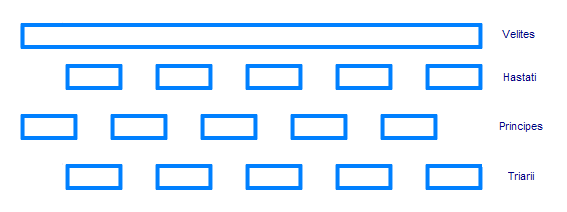
\includegraphics[width=\linewidth]{../ressources/Polybian_formation}
	\caption{Disposition classique en trois lignes \cite{roman_infantry_tactics}}
	\end{centering}
\end{figure}
\begin{figure}[H]
	\begin{centering}
	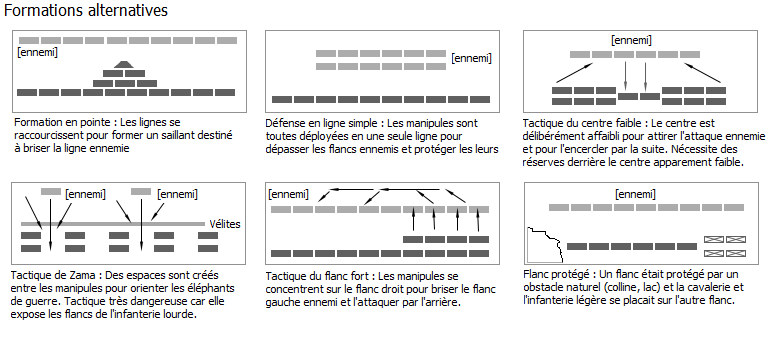
\includegraphics[width=\linewidth]{../ressources/Formations_infanterie_romaine}
	\caption{Formations alternatives \cite{roman_infantry_tactics}}
	\end{centering}
\end{figure}



\subsection{Tactiques}

\subsubsection{Charge}
\begin{figure}[H]
	\begin{centering}
	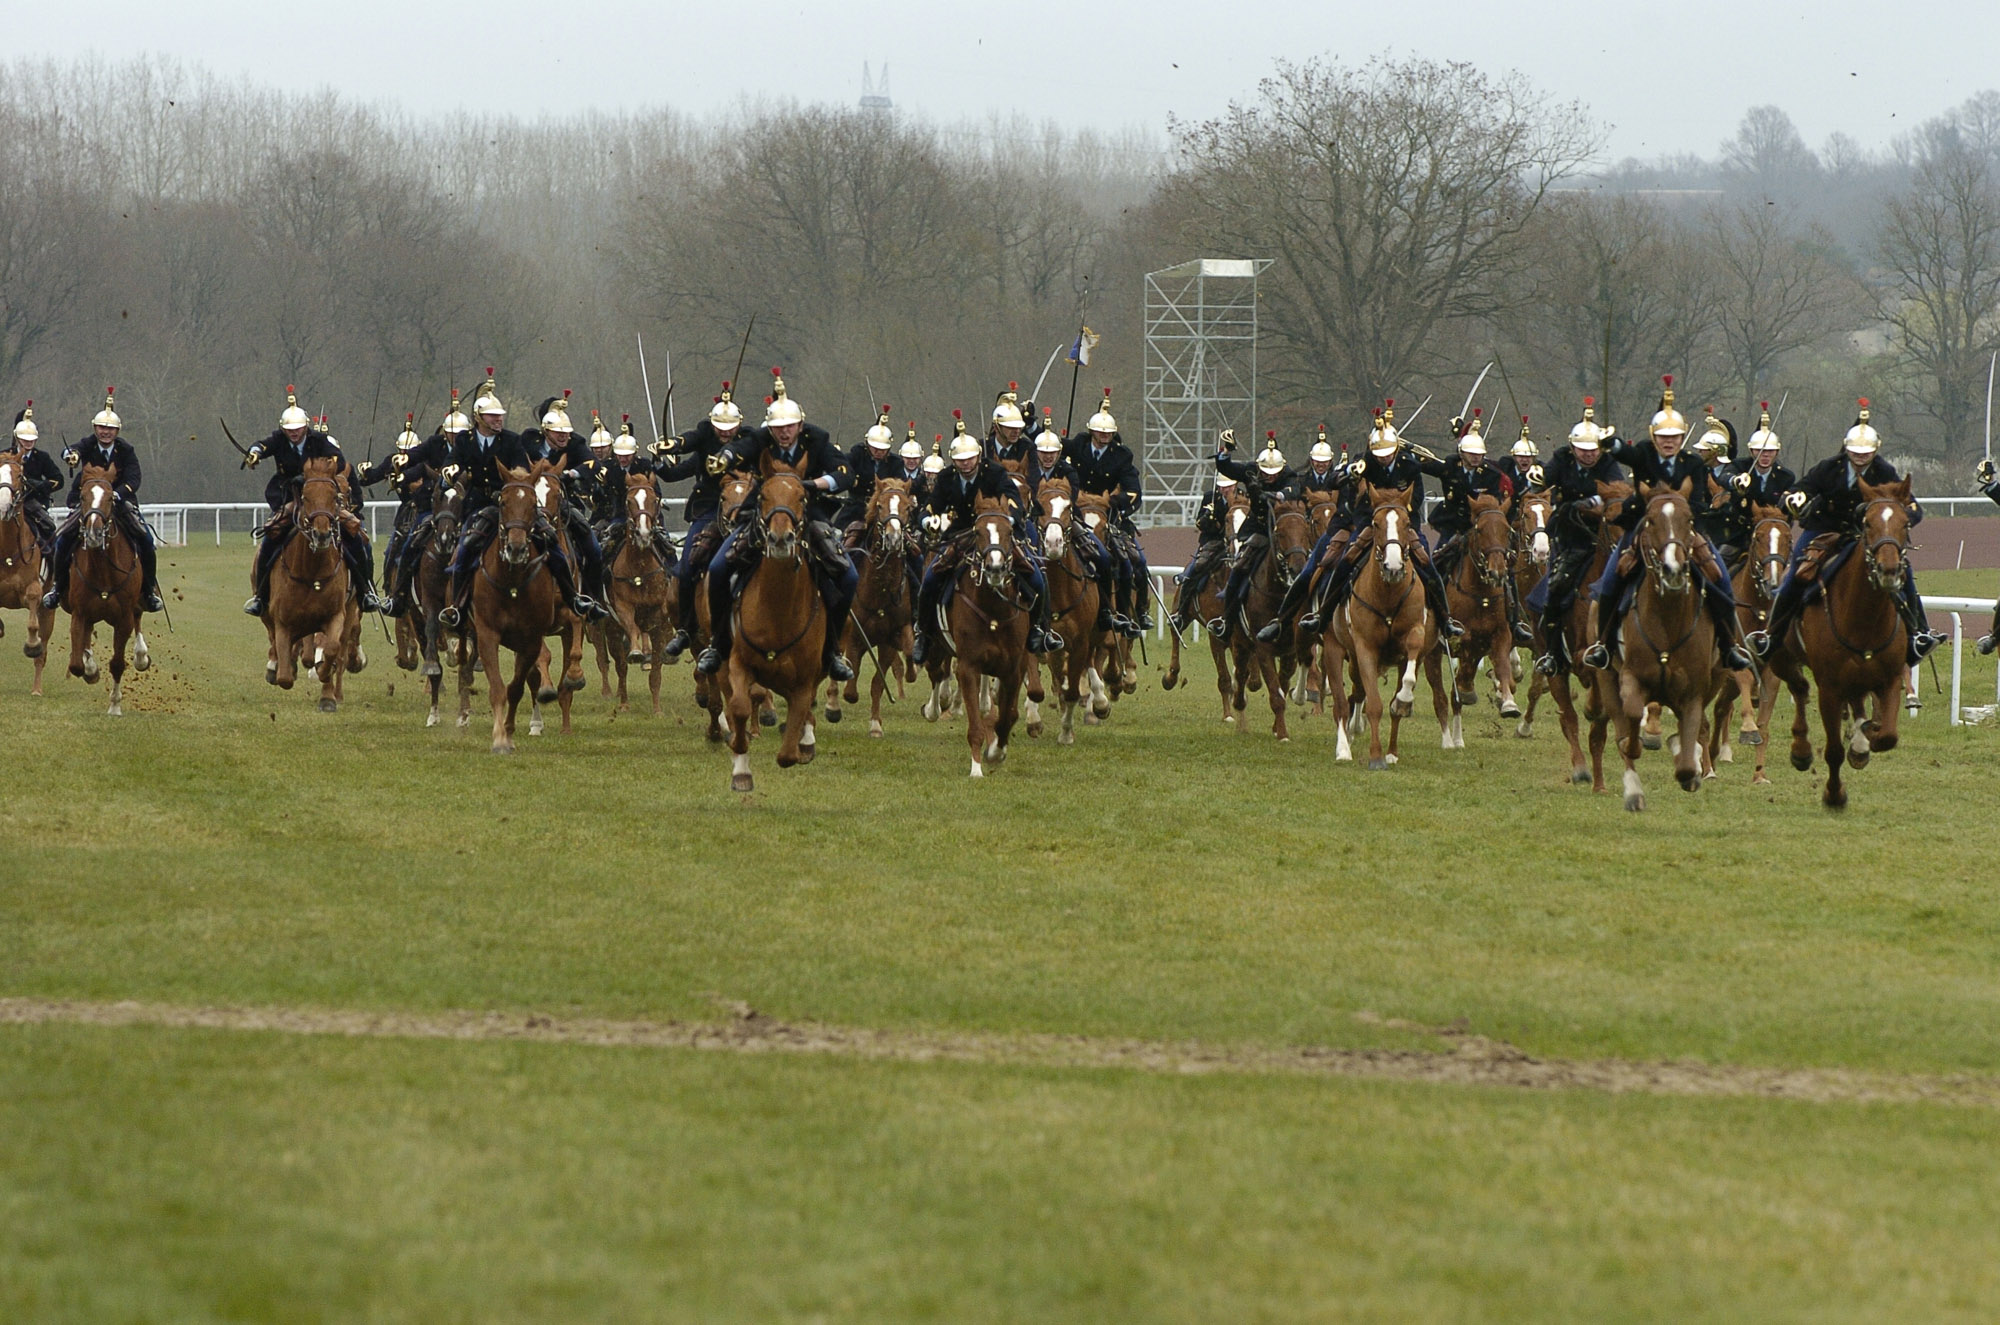
\includegraphics[width=\linewidth]{../ressources/Charge-de-cavalerie}
	\caption{Charge de cavalerie de la garde républicaine \cite{charge_cavalery}}
	\end{centering}
\end{figure}
\begin{figure}[H]
	\begin{centering}
	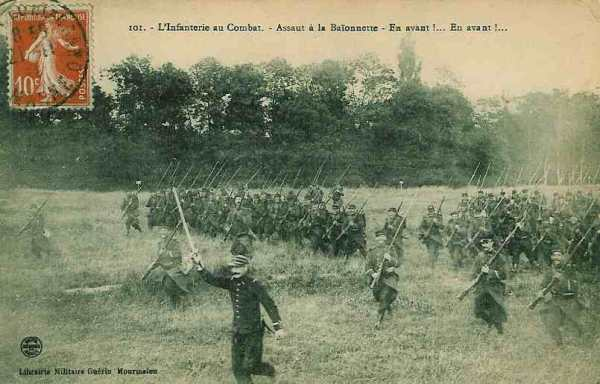
\includegraphics[width=\linewidth]{../ressources/charge_infanterie}
	\caption{Charge d’infanterie française 1914 \cite{infantery_charge}}
	\end{centering}
\end{figure}
\cite{charge_tactic}

\subsubsection{Manœuvre de flanquement}
\begin{figure}[H]
	\begin{centering}
	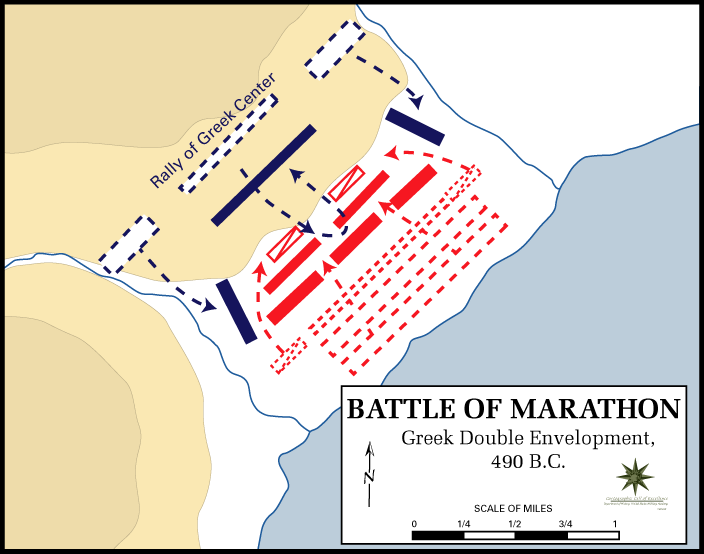
\includegraphics[width=\linewidth]{../ressources/Battle_of_Marathon}
	\caption{Bataille de Marathon (double enveloppement, manœuvre de flanquement) \cite{flanking_maneuver}}
	\end{centering}
\end{figure}
\begin{figure}[H]
	\begin{centering}
	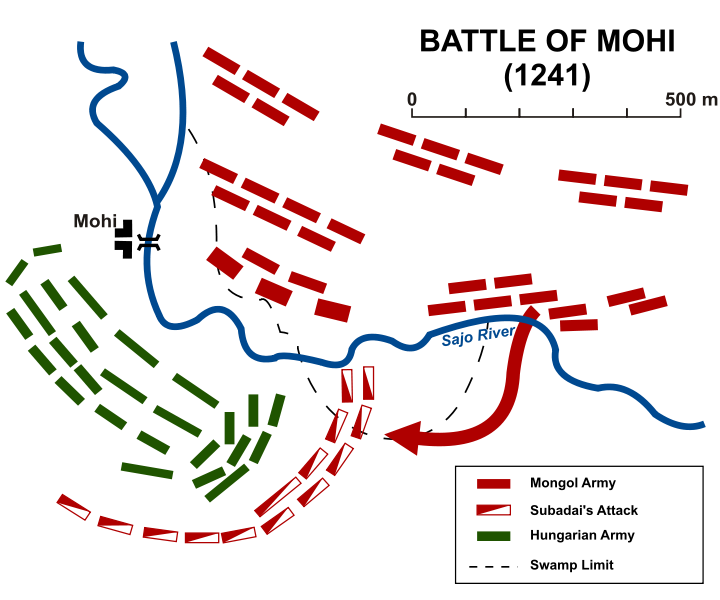
\includegraphics[width=\linewidth]{../ressources/Battle_of_Mohi}
	\caption{Plan de la bataille de Mohi (Hongrie) \cite{mohi_battle}}
	\end{centering}
\end{figure}
\cite{tactic,pincer_tactic}

\subsubsection{Le marteau et l'enclume}
\begin{figure}[H]
	\begin{centering}
	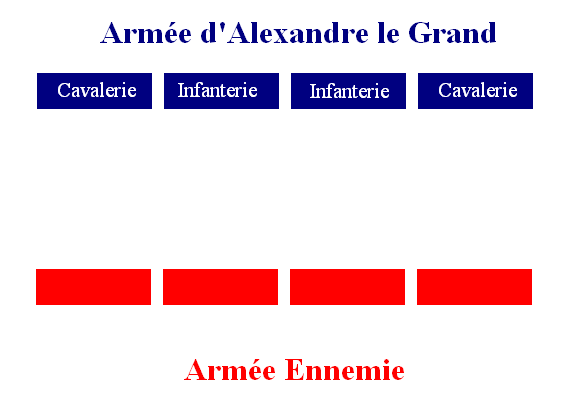
\includegraphics[width=0.8\linewidth]{../ressources/marteau}
	\caption{}
	\end{centering}
\end{figure}
\begin{figure}[H]
	\begin{centering}
	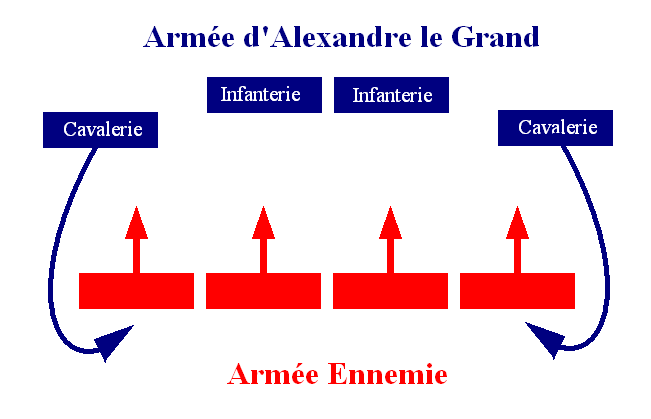
\includegraphics[width=0.8\linewidth]{../ressources/marteau2}
	\caption{}
	\end{centering}
\end{figure}
\begin{figure}[H]
	\begin{centering}
	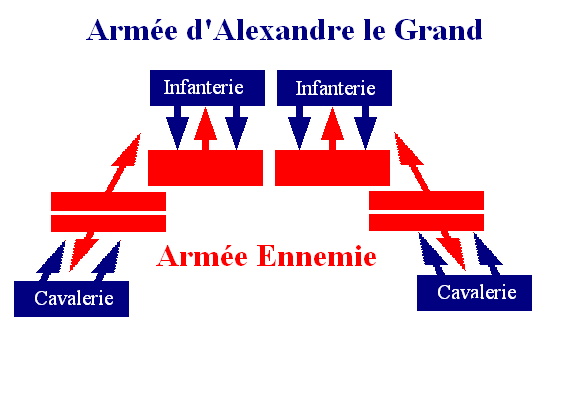
\includegraphics[width=0.8\linewidth]{../ressources/enclume}
	\caption{}
	\end{centering}
\end{figure}
\begin{figure}[H]
	\begin{centering}
	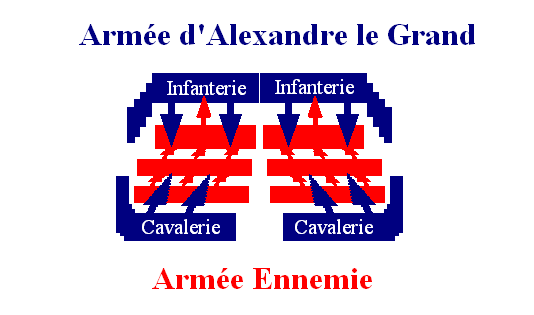
\includegraphics[width=0.8\linewidth]{../ressources/enclume2}
	\caption{}
	\end{centering}
\end{figure}
\cite{Alexanders_tactics}

\subsubsection{Contre-attaque}
\begin{figure}[H]
	\begin{centering}
	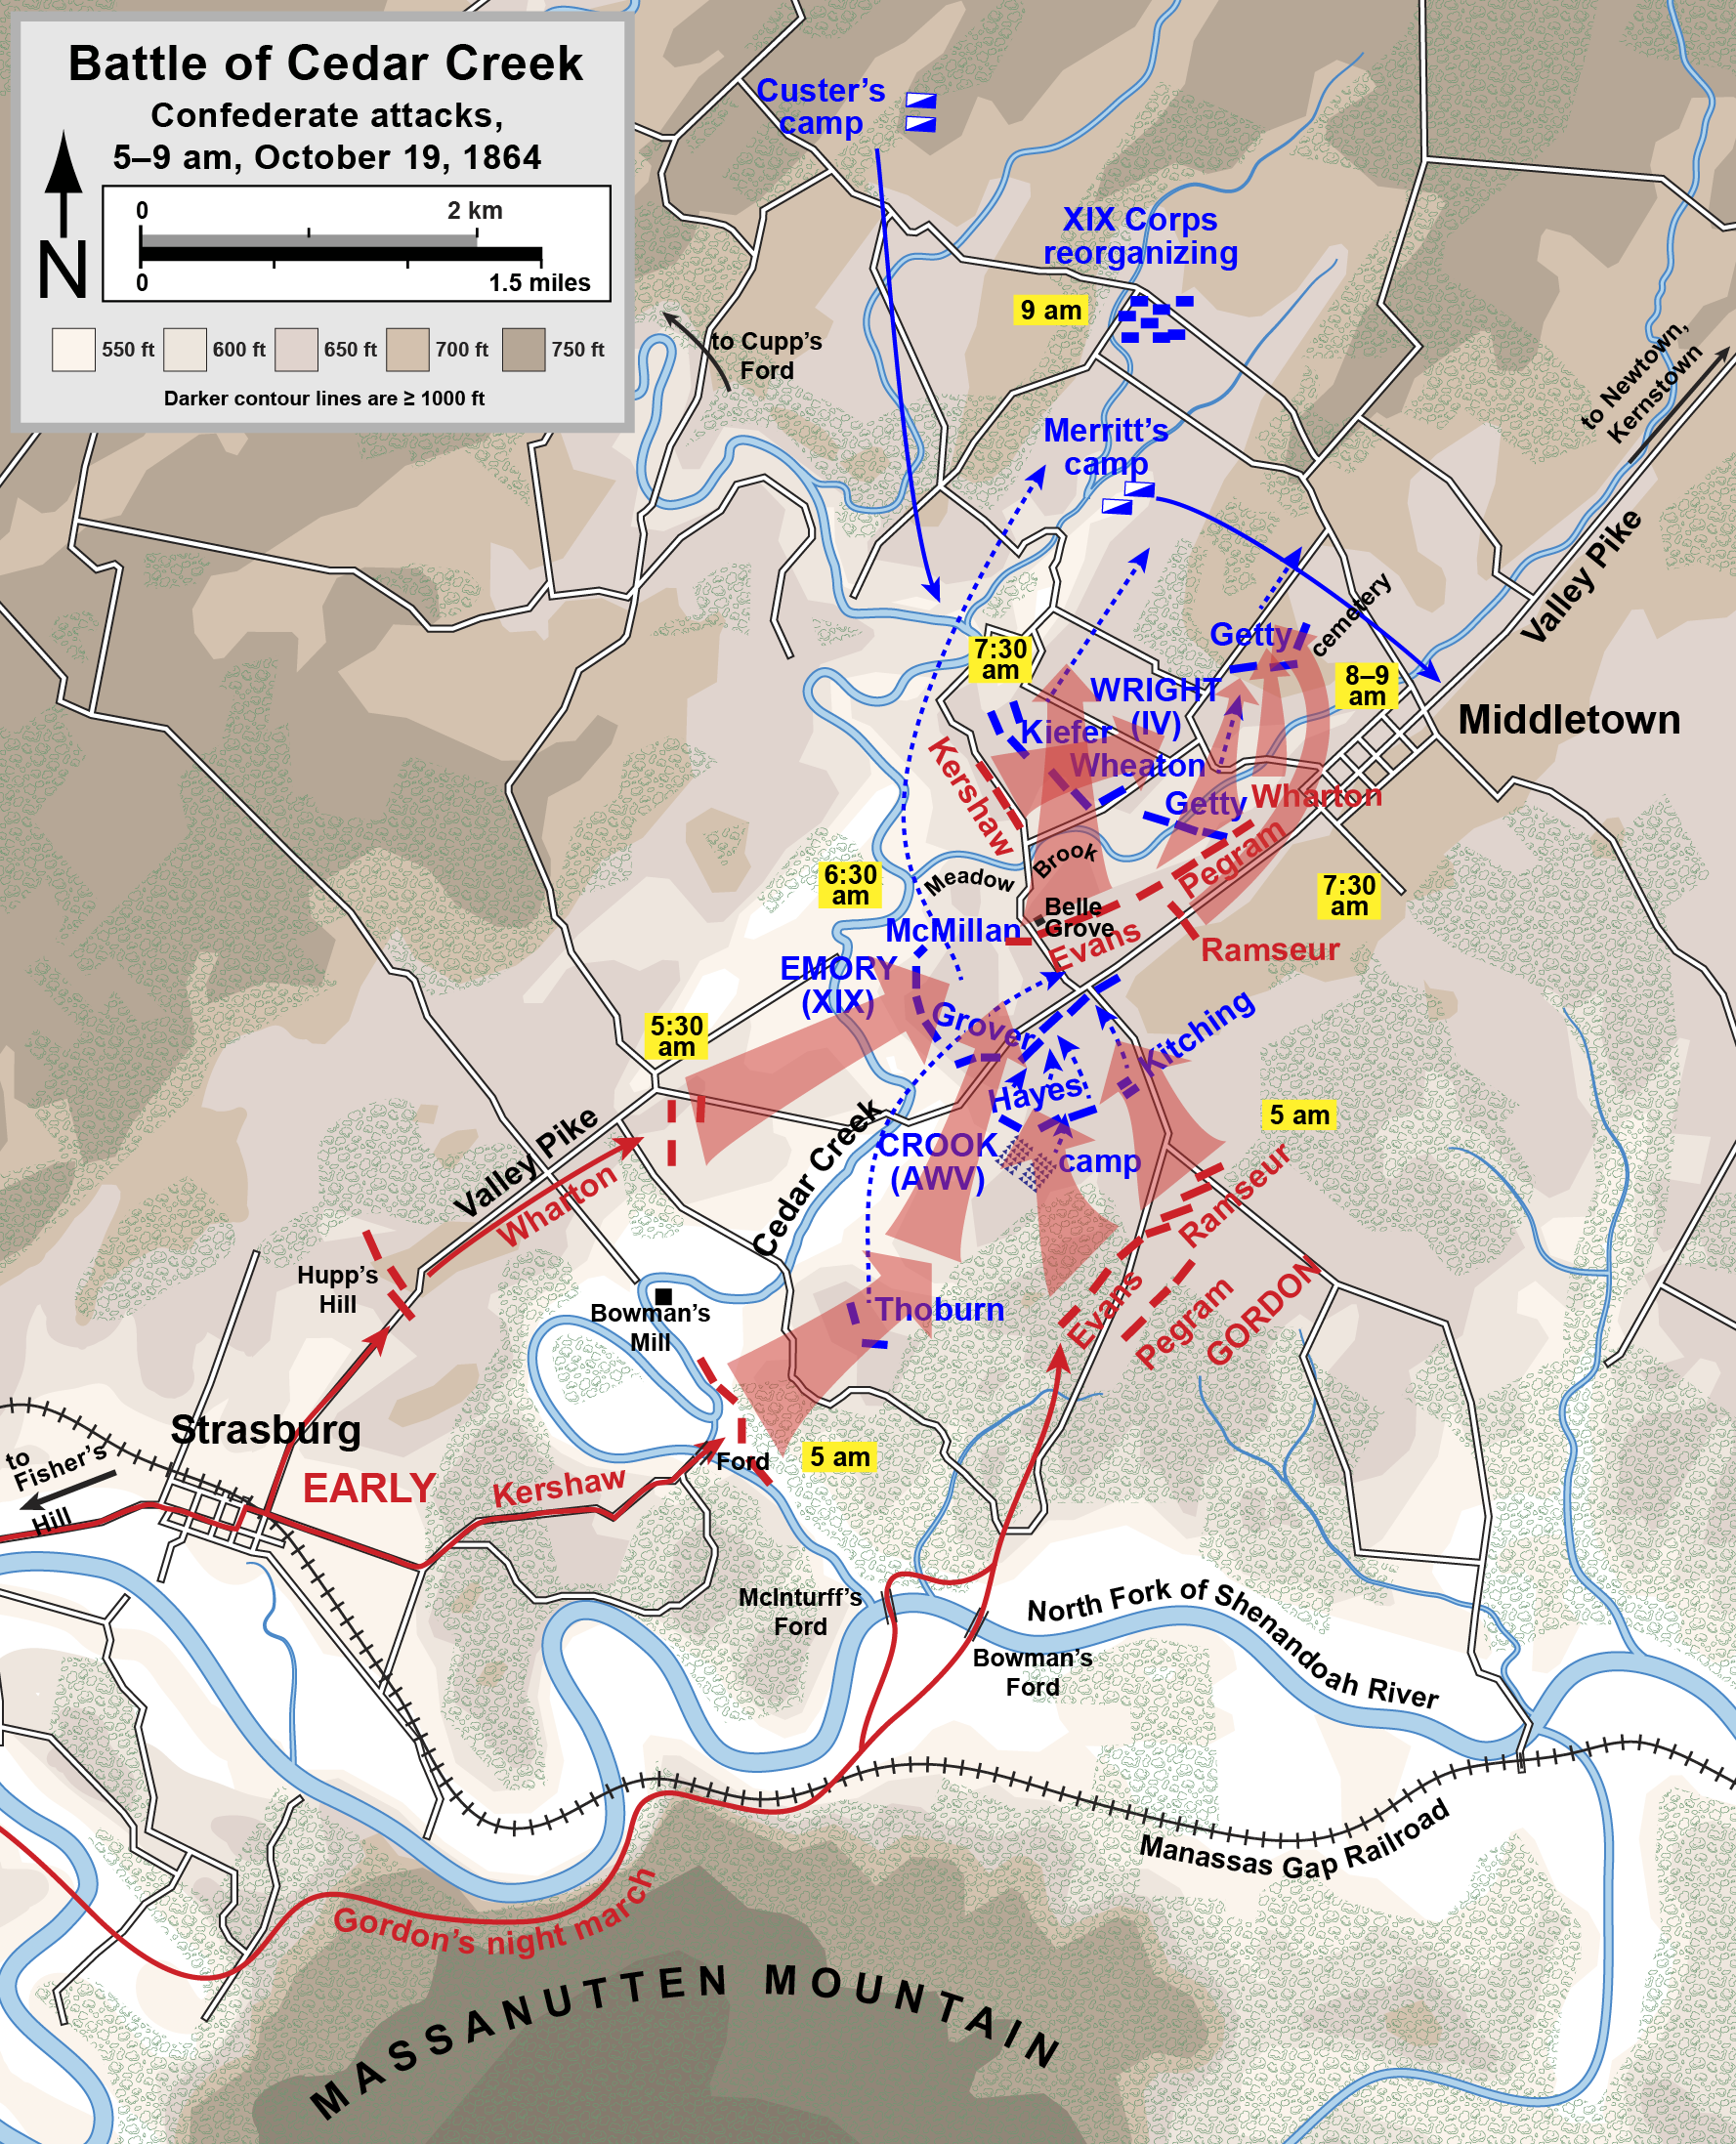
\includegraphics[width=\linewidth]{../ressources/Cedar_Creek_Confederate_attacks}
	\caption{Battle of Cedar Creek, Confederate attacks}
	\end{centering}
\end{figure}
\begin{figure}[H]
	\begin{centering}
	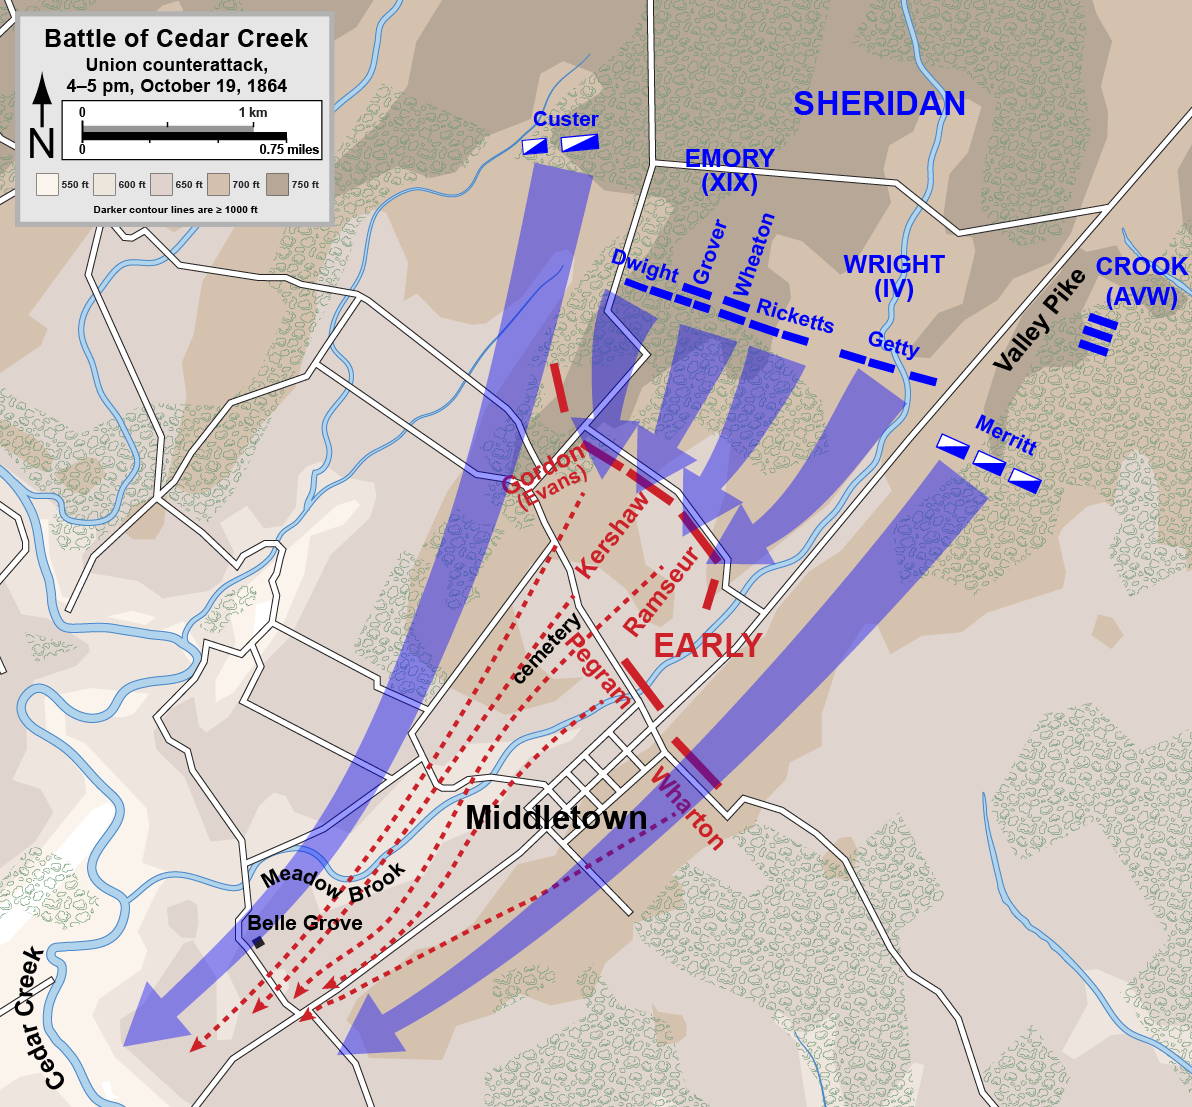
\includegraphics[width=\linewidth]{../ressources/Cedar_Creek_Union_counterattack}
	\caption{Battle of Cedar Creek, Union counterattack}
	\end{centering}
\end{figure}
\cite{counterattack_wiki, couterattack_cedar_creek}

\subsubsection{Retraite feinte}
\begin{figure}[H]
	\begin{centering}
	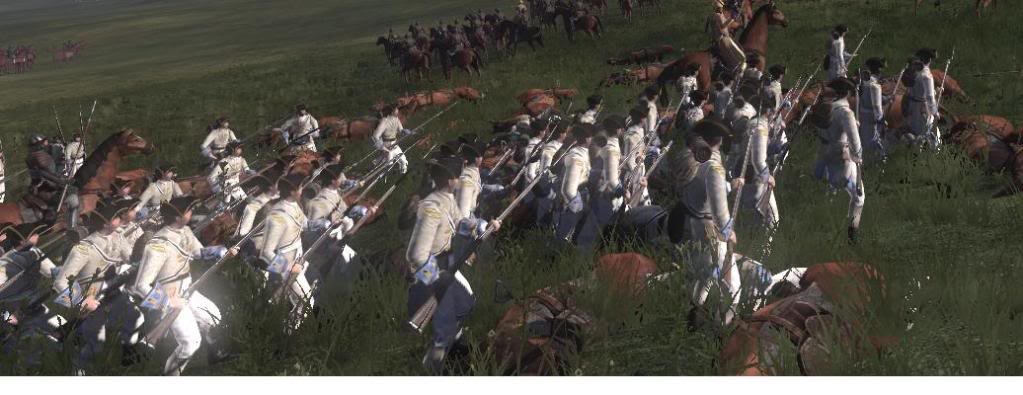
\includegraphics[width=\linewidth]{../ressources/infantrysquare3}
	\caption{These French troops broke formation, and are pursuing the enemy cavalry. \cite{feigned_retreat}}
	\end{centering}
\end{figure}
\cite{mongol_army}


\subsubsection{Embuscade}
\begin{figure}[H]
	\begin{centering}
	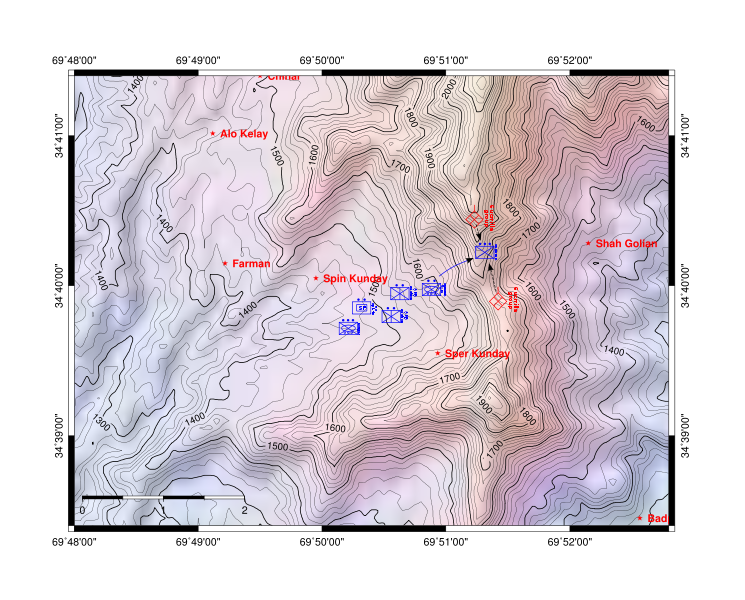
\includegraphics[width=\linewidth]{../ressources/Uzbin_valley_ambush-map}
	\caption{Embuscade d'Uzbin \cite{uzbin_ambush}}
	\end{centering}
\end{figure}
\begin{figure}[H]
	\begin{centering}
	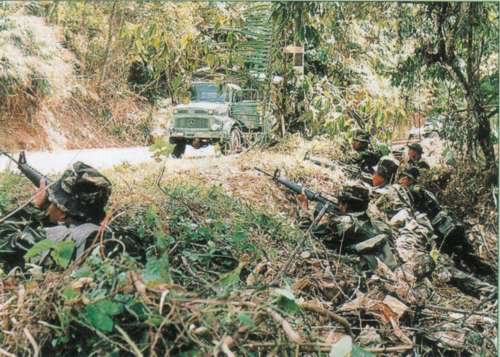
\includegraphics[width=0.8\linewidth]{../ressources/ambush}
	\caption{Malaysian Armed Forces ambush \cite{ambush_picture}}
	\end{centering}
\end{figure}
\cite{ambush_wiki}

\subsubsection{Hit and run}




\section{Applications aux systèmes multi-agents}

\subsection{Enhanced Isaac Neural Simulation Toolkit (EINSTein)}
an Artificial-Life Laboratory for Exploring Self-Organized Emergence in Land Combat
\begin{figure}[H]
	\begin{centering}
	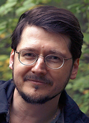
\includegraphics[]{../ressources/ilachinski}
	\caption{Andy Ilachinski}
	\end{centering}
\end{figure}
1999
\begin{figure}[H]
	\begin{centering}
	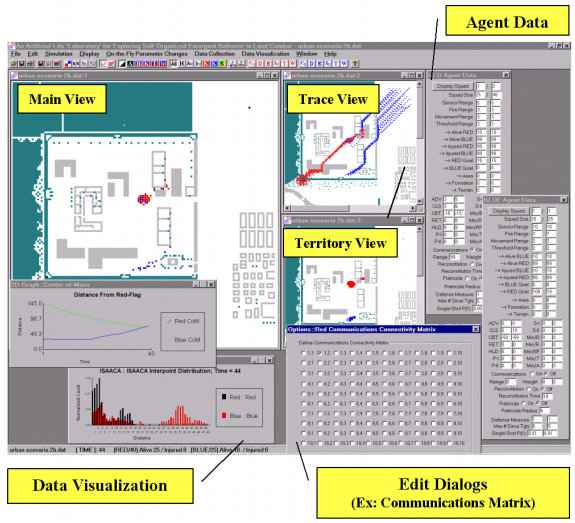
\includegraphics[width=\linewidth]{../ressources/Einstein}
	\caption{}
	\end{centering}
\end{figure}
\cite{simu_guerre,ilachinski1994,ilachinski1999}

motivation des agents
\begin{figure}[H]
	\begin{centering}
	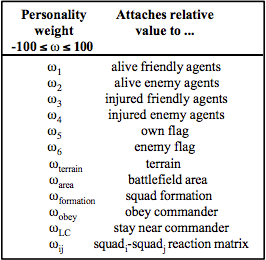
\includegraphics[]{../ressources/einstein_personality_weight}
	\caption{}
	\end{centering}
\end{figure}
\begin{figure}[H]
	\begin{centering}
	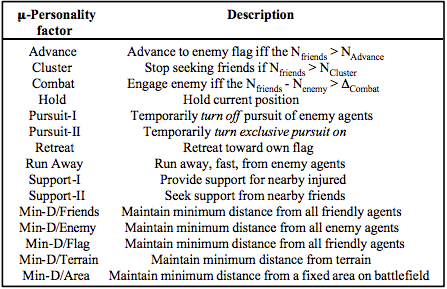
\includegraphics[]{../ressources/einstein_personality_factor}
	\caption{}
	\end{centering}
\end{figure}

émergence d'un comportement global
\begin{figure}[H]
	\begin{centering}
	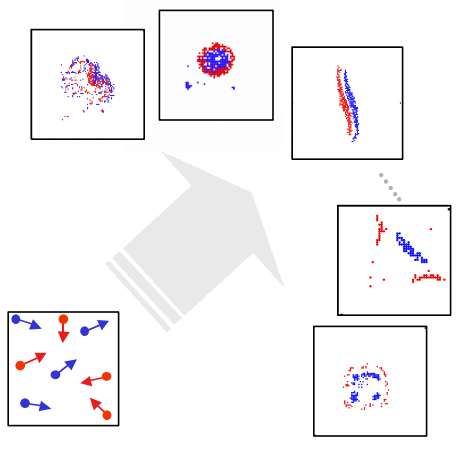
\includegraphics[width=0.8\linewidth]{../ressources/einstein_global_behavior}
	\caption{}
	\end{centering}
\end{figure}
formation en pointe
encerclement
assault frontal
prise en tenaille
guérilla

\subsection{Iruba}
An Agent-Based Model of the Guerrilla War Process
\begin{figure}[H]
	\begin{centering}
	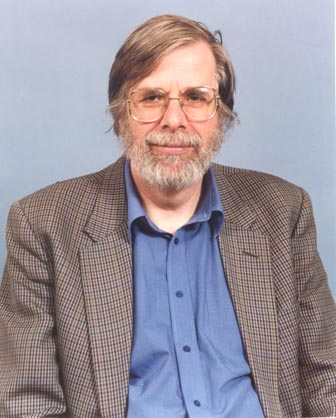
\includegraphics[]{../ressources/doran}
	\caption{Jim Doran}
	\end{centering}
\end{figure}
2005
\begin{figure}[H]
	\begin{centering}
	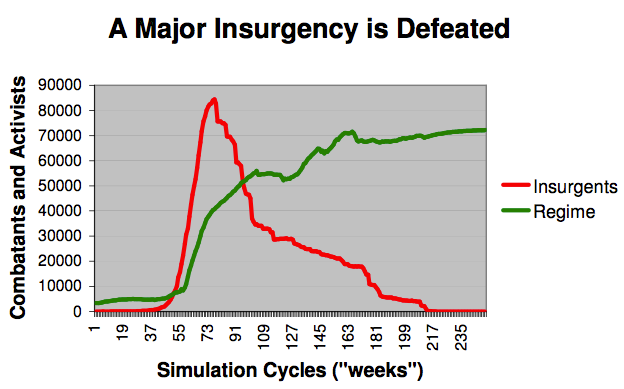
\includegraphics[width=\linewidth]{../ressources/insurgency}
	\caption{}
	\end{centering}
\end{figure}
\begin{algorithmic}[1]
		\WHILE{non termination}
			\STATE Attacks and their impact
			\STATE HQ decisions
			\STATE Recruitment
			\STATE Force movement
		\ENDWHILE
		\end{algorithmic}
\cite{doran2005iruba}

Stratégies influant sur la réussite
initial guerrilla band size
regime force concentration
insurgent mobility
insurgent hyper-mobility
all-out regime counter attack

Stratégies influant sur la réussite
\begin{figure}[H]
	\begin{centering}
	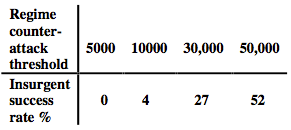
\includegraphics[scale=0.9]{../ressources/iruba_counter_attack}
	\caption{}
	\end{centering}
\end{figure}
\begin{figure}[H]
	\begin{centering}
	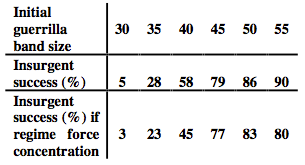
\includegraphics[scale=0.9]{../ressources/iruba_force_concentration}
	\caption{}
	\end{centering}
\end{figure}
\begin{figure}[H]
	\begin{centering}
	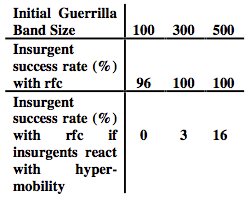
\includegraphics[scale=0.9]{../ressources/iruba_hyper_mobility}
	\caption{}
	\end{centering}
\end{figure}
\begin{figure}[H]
	\begin{centering}
	\includegraphics[scale=0.9]{../ressources/iruba_mobility}
	\caption{}
	\end{centering}
\end{figure}

\subsection{RPDAgent}
Enhanced Military Decision Modeling Using a MultiAgent System Approach
\begin{figure}[H]
	\begin{centering}
	\includegraphics[scale=0.5]{../ressources/john_sokolowski}
	\caption{John A. Sokolowski}
	\end{centering}
\end{figure}
2003
\begin{figure}[H]
	\begin{centering}
	\includegraphics[scale=0.9]{../ressources/RPDagent_uml}
	\caption{}
	\end{centering}
\end{figure}
\cite{sokolowski2003}


\section{Conclusion}


\newpage
\bibliographystyle{plain}
\bibliography{../Bib.bib}

\end{document}


